\documentclass{article}
\usepackage[utf8]{inputenc}
\usepackage[a4paper, margin=1in]{geometry}
\usepackage{amsmath}
\usepackage{amssymb}
\usepackage{graphicx}
\usepackage{url}
\usepackage{hyperref}
\newcommand{\algorithmautorefname}{Algorithm}
\usepackage{algorithm}
\usepackage[noend]{algpseudocode}
\usepackage{subcaption}

\linespread{1.5}

\renewcommand{\algorithmicforall}{\textbf{for each}}
\newcommand{\algorithmicbreak}{\textbf{break}}
\newcommand{\Break}{\State \algorithmicbreak}
\newcommand{\Continue}{\State \textbf{continue}}
\renewcommand{\Comment}[1]{\hfill\textit{$\triangleright$ #1}}

\title{Selected Methods in $N$-body Simulations}
\author{Aleksy Bałaziński}
\date{\today}

\begin{document}

\newcommand{\PThreeM}{P$^3$M}

\maketitle

\tableofcontents

\section{Introduction}
The dominant force over large distances is the gravitational force.
The force exerted on a body with mass $m_2$ at the point $\mathbf{x}_2$ by a body with mass $m_1$ located at $\mathbf{x}_1$ can be expressed by the relation
\begin{equation*}\label{eq:law-of-uni-grav}
    \mathbf{F} = -G\frac{m_1m_2}{|\mathbf{x}_{21}|^3}\mathbf{x}_{21}
\end{equation*}
where $G$ is the gravitational constant $6.674\times 10^{-11} \mathrm{m}^3  \mathrm{kg}^{-1}\mathrm{s}^{-2}$ and $\mathbf{x}_{21} = \mathbf{x}_2 - \mathbf{x}_1$.
Therefore, the evolution of a system of $N$ bodies is described by $N$ equations
\begin{equation}\label{eq:pp-method}
    \ddot{\mathbf{x}}_i = -G\sum_{j\neq i} \frac{m_j}{|\mathbf{x}_{ij}|^3}\mathbf{x}_{ij}.
\end{equation}
for each $i = 1,\dots, N$.
Direct application of \autoref{eq:pp-method} is the basis the so-called \textit{particle-particle} method.
The method is characterized by $O(N^2)$ time complexity (more precisely, it requires $(N-1)N/2$ operations if Newton's 3rd law is used in the computation).
Assuming that 100ns are required to perform the floating-point operations under the summation symbol, $N=30,000$, and 150 iterations, the simulation would take approximately 2 hours to complete.
It is therefore evident that more efficient algorithms have to be put in place in order to make simulations of this scale feasible.

The \textit{particle-mesh} (PM) technique, introduced around 1985 by Hockney and Eastwood, was an early improvement over the PP method.
In the PM approach, the space is divided into a rectangular grid (or mesh) of cells.
Each cell is assigned a portion of the mass of nearby particles, creating a density distribution $\rho(\mathbf{x})$.
The relation between the density and gravitational potential $\phi$, in the form of Poisson's equation
\begin{equation}\label{eq:poisson}
    \nabla^2\phi = 4\pi G \rho,
\end{equation}
is then used to obtain the potential at each cell center.
The gravitational field $\mathbf{g}$ can then be calculated as $\mathbf{g} = -\nabla \phi$.
Since $\mathbf{g}$ equals the acceleration due to gravity, we get $\ddot{\mathbf{x}}_i = \mathbf{g}(\mathbf{x}_i)$.

The drawback of the PM method is its poor modeling of forces over short distances.
Eastwood and Hockney proposed a remedy for this problem: the \textit{particle-particle-particle-mesh} method (or \PThreeM{} in short).
In the \PThreeM{} method, the force on the $i$-th particle is split into two components: \textit{short-range} and \textit{long-range} force.
The long-range force is calculated using the PM method, whereas the short-range force can be found by direct summation of the forces due to nearby particles.

The computational complexity of the PM and \PThreeM{} methods depends on the implementation of the potential solver used to calculate $\phi$ from \autoref{eq:poisson}.
For instance, if a fast Fourier transform is used, then the complexity of the PM algorithm is $O(N + N_g^3\log N_g)$, where $N_g$ is the number of cells in a single dimension of the grid (note it is linear in $N$).
For the \PThreeM{} method, the worst-case scenario happens when all particles are clustered closely together, which causes the short-range $O(N^2)$ correction part to become dominant.

\section{Particle-mesh method}
The particle-mesh method can be described as the following sequence of four steps:
\begin{enumerate}
    \item Assign masses to mesh points,
    \item Solve the field equation (\autoref{eq:poisson}) on the mesh,
    \item Calculate the field strength at mesh-points,
    \item Find forces applied to individual particles by interpolation.
\end{enumerate}
In this section, each of these steps will be described in more detail.

\subsection{Mass assignment}\label{subsec:mass-assignment}
The specifics of assigning mass from particles to mesh points depend on the density profile (or \textit{shape}) associated with the particles.
In general, the particles need not be represented as idealized dimensionless points;
indeed, it is possible to construct a hierarchy of shapes, where each successive member covers a larger number of mesh points and whose application leads to smaller numerical errors.

An infinite hierarchy of shapes with this property, as described by Hockney and Eastwood in \cite{Hockney1988}, can be generated by successive convolutions with the ``top-hat'' function $\Pi$, defined as
\begin{equation*}
    \Pi(x) = \begin{cases}
        1,           & |x| < \frac{1}{2} \\
        \frac{1}{2}, & |x| = 1           \\
        0,           & \text{otherwise}.
    \end{cases}
\end{equation*}
The three most popular assignment schemes that hail from this family (and the ones implemented in our program) are the \textit{nearest grid point} (NGP), \textit{cloud in cell} (CIC), and \textit{triangular shaped cloud} (TSC) schemes, with shapes $S$ given by
\begin{align*}
    S_\text{NGP} & = \delta(x), & S_\text{CIC} & = \delta(x) * \frac{1}{H} \Pi\left(\frac{x}{H}\right) = \frac{1}{H}\Pi\left(\frac{x}{H}\right), & S_\text{TSC} & = \frac{1}{H}\Pi\left(\frac{x}{H}\right) * \frac{1}{H}\Pi\left(\frac{x}{H}\right) = \frac{1}{H}\Lambda \left(\frac{x}{H}\right),
\end{align*}
where $\Lambda$ is the triangle function
\begin{equation*}
    \Lambda(x) = \begin{cases}
        1 - |x|, & |x| < 1           \\
        0,       & \text{otherwise}.
    \end{cases}
\end{equation*}
For illustrative purposes, the shape $S_\text{CIC}$ is depicted in \autoref{fig:cic-shape}.
\begin{figure}[htp]
    \centering
    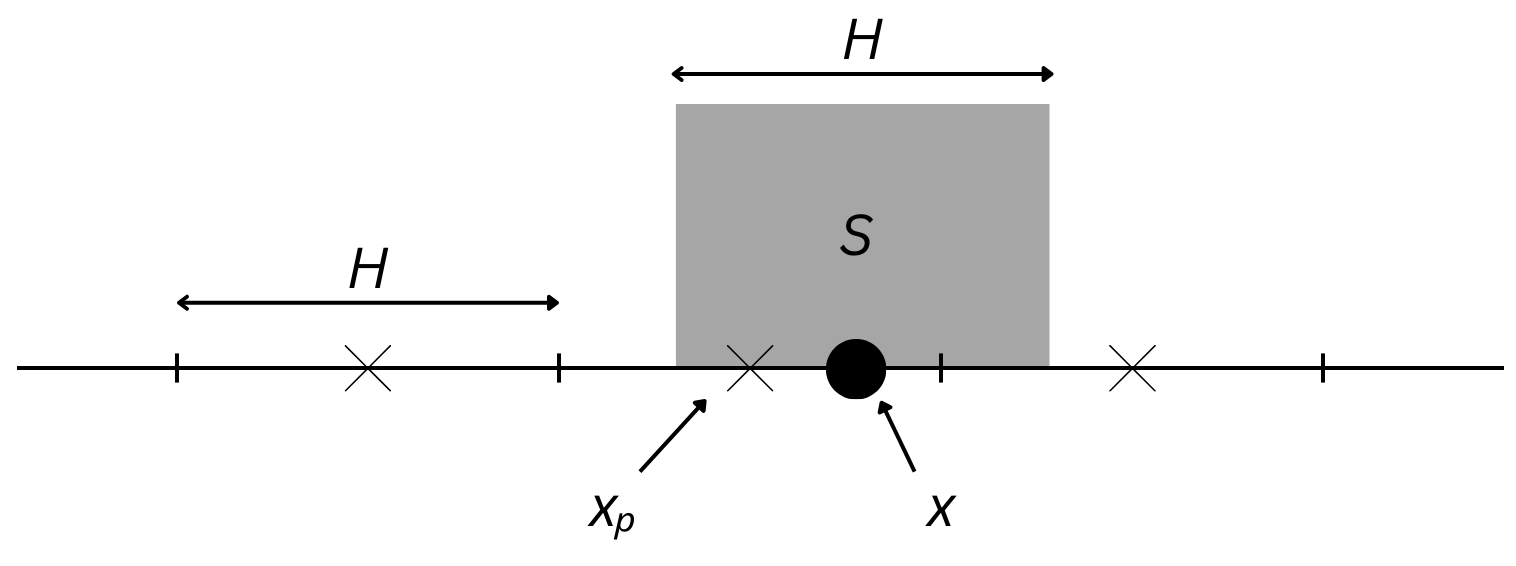
\includegraphics[scale=0.2]{img/CIC.png}
    \caption{The CIC shape centered at $x$ (particle position).
        The particle is within cell $x_p$, however, the cell $x_{p+1}$ gets non-zero density contribution from the particle.}
    \label{fig:cic-shape}
\end{figure}

In the one-dimensional case, the fraction of mass $W_p$ assigned to mesh-point $p$ from particle at position $x$ is given by
\begin{equation*}
    W(x-x_p) = W_p(x) = \int_{x_p-H/2}^{x_p+H/2} S(x'-x)dx'.
\end{equation*}
A simple rule for relating the assignment function $W$ defined above with shape $S$ can be found by noticing that
\begin{equation*}
    W(x) = \int_{-H/2}^{H/2}S(x'-x)dx' = \int_{-\infty}^\infty \Pi\left(\frac{x'}{H}\right)S(x'-x)dx' = \Pi\left(\frac{x}{H}\right) * S(x).
\end{equation*}
This implies that
\begin{align}\label{eq:assignment-functions}
    W_\text{NGP}(x) & = \Pi\left(\frac{x}{H}\right), & W_\text{CIC}(x) & = \Lambda\left(\frac{x}{H}\right), & W_\text{TSC}(x) & = \Pi\left(\frac{x}{H}\right) * \frac{1}{H} \Lambda\left(\frac{x}{H}\right) = (\Pi * \Lambda)\left(\frac{x}{H}\right).
\end{align}
Splitting the domain of integration in the expression for $W_\text{TSC}$ into five disjoint intervals shows that
\begin{equation*}
    (\Pi * \Lambda)(x) = \begin{cases}
        \frac{1}{8}(3-2|x|)^2, & \frac{1}{2} \leq |x| < \frac{3}{2} \\
        \frac{3}{4}-x^2,       & |x| < \frac{1}{2}                  \\
        0,                     & \text{otherwise}.
    \end{cases}
\end{equation*}

Two- and three-dimensional versions of the assignment functions in \autoref{eq:assignment-functions} are products of the assignment functions in each dimension.
For example, the three-dimensional assignment function $W$ is
\begin{equation*}
    W(\mathbf{x}) = W(x)W(y)W(z).
\end{equation*}
Hence, the mass assigned at mesh-point at $\mathbf{x}_\mathbf{p}$ is
\begin{equation*}
    m(\mathbf{x}_\mathbf{p}) = \sum_i m_i W_\mathbf{p}(\mathbf{x}_i),
\end{equation*}
or, in terms of density $\rho$,
\begin{equation}\label{eq:density-assignment}
    \rho(\mathbf{x}_\mathbf{p}) = \frac{1}{V} \sum_i m_i W_\mathbf{p}(\mathbf{x}_i),
\end{equation}
where $V = H^3$ is the volume of a cell and $i$ indexes the particles.

Obviously, \autoref{eq:density-assignment} is not suitable for direct application in the actual algorithm.
Instead, we iterate over all particles, identify the parent cell $\mathbf{p}$ of each particle (and its neighborhood) and update $\rho$.
This process is illustrated in \autoref{alg:density-assignment}.
\begin{algorithm}
    \caption{Density assignment algorithm}\label{alg:density-assignment}
    \begin{algorithmic}[1]
        \ForAll {particle $i$}
        \ForAll {cell $\mathbf{q}$ in $\mathcal{C}_S(\mathbf{x}_i)$}
        \State $\rho(\mathbf{x}_\mathbf{q}) \gets \rho(\mathbf{x}_\mathbf{q}) + m_i W(\mathbf{x}_i - \mathbf{x}_\mathbf{q}) / V$
        \EndFor
        \EndFor
    \end{algorithmic}
\end{algorithm}
The set $\mathcal{C}_S(\mathbf{x}_i)$ of cells that have to be considered while assigning density from the $i$-th particle, depends on the shape $S$ of the particle.
Specifically, we have $\mathcal{C}_\mathrm{NGP}(\mathbf{x}) = \{[\mathbf{x} / H]\}$, $\mathcal{C}_\mathrm{CIC}(\mathbf{x}) = \{\lfloor \mathbf{x}/H \rfloor + \mathbf{t} \;|\; t_i =0,1\}$, and $\mathcal{C}_\mathrm{TSC}(\mathbf{x}) = \{[\mathbf{x} / H] + \mathbf{t} \;|\; t_i = -1, 0, 1\}$.
It follows that $|\mathcal{C}_\mathrm{NGP}(\mathbf{x})| = 1$, $|\mathcal{C}_\mathrm{CIC}(\mathbf{x})| = 8$, and $|\mathcal{C}_\mathrm{TSC}(\mathbf{x})| = 27$ which illustrates the increasing computational cost resulting from using higher-order assignment schemes.
We note that \autoref{alg:density-assignment} can be parallelized if atomic increments are used in line 3.

\subsection{Solving the field equation}
The Poisson equation (\autoref{eq:poisson}) can be restated in integral form
\begin{equation*}
    \phi(\mathbf{x}) = \int \mathcal{G}(\mathbf{x}-\mathbf{x}')\rho(\mathbf{x}') dV',
\end{equation*}
which has the following discrete analogue
\begin{equation}\label{eq:poisson-discrete}
    \phi(\mathbf{x}_\mathbf{p}) = V \sum_{\mathbf{p}'} \mathcal{G}(\mathbf{x}_\mathbf{p} - \mathbf{x}_{\mathbf{p}'}) \rho(\mathbf{x}_{\mathbf{p}'}),
\end{equation}
where $\mathcal{G}$ is the Green's function (potential due to unit mass).
The right-hand side of \autoref{eq:poisson-discrete} is a convolution sum that runs over a finite set of mesh points.
If we assume periodic boundary conditions, we can apply the discrete Fourier transform to both sides and use the convolution theorem to conclude that\footnote{
    In this work, the Hockney \& Eastwood definition of DFT is used, i.e.
    \begin{equation*}
        D(x_p) = \frac{1}{L}\sum_{l=0}^{N-1}\hat{D}(k)e^{ikx_p}, \quad \hat{D}(k) = H\sum_{p=0}^{N-1}D(x_p)e^{-ikx_p},
    \end{equation*}
    where $x_p = pH$.
    The conversion between this form and another popular definition,
    \begin{equation}\label{eq:standard-dft}
        \widetilde{D_H}(k) = \sum_{p=0}^{N-1}D_H(p)e^{-i2\pi kp / N},
    \end{equation}
    is given by
    \begin{equation*}
        \widetilde{D_H}(k) = \frac{1}{H}\hat{D}\left(\frac{2\pi}{NH}k\right),
    \end{equation*}
    where $D_H(p) = D(pH)$.
}
\begin{equation}\label{eq:poisson-fourier-product}
    \hat{\phi}(\mathbf{k}) = \hat{\mathcal{G}}(\mathbf{k}) \hat{\rho}(\mathbf{k}).
\end{equation}

An approximation to $\hat{\mathcal{G}}$ can be found using a discretized version of the Laplacian in \autoref{eq:poisson-discrete}.
Specifically, for a 7-point stencil,
\begin{equation*}
    \begin{split}
        4\pi G\rho(\mathbf{x}_{ijk})
         & =\frac{\phi(\mathbf{x}_{i-1,j,k}) - 2\phi(\mathbf{x}_{ijk})+\phi(\mathbf{x}_{i+1,j,k})}{H^2}   \\
         & + \frac{\phi(\mathbf{x}_{i,j-1,k}) - 2\phi(\mathbf{x}_{ijk})+\phi(\mathbf{x}_{i,j+1,k})}{H^2}  \\
         & + \frac{\phi(\mathbf{x}_{i,j,k-1}) - 2\phi(\mathbf{x}_{ijk})+\phi(\mathbf{x}_{i,j,k+1})}{H^2}.
    \end{split}.
\end{equation*}
Applying the discrete Fourier transform to both sides and using the shift theorem we get
\begin{align*}
    4\pi G \hat{\rho}(\mathbf{k})
     & = \frac{1}{H^2}\sum_{i=1}^{3}\left( e^{-iHk_i} + e^{iHk_i}-2 \right)\hat{\phi}(\mathbf{k})       \\
     & = \frac{1}{H^2} \sum_{i=1}^{3}\left( e^{iHk_i/2} - e^{-iHk_i/2} \right)^2 \hat{\phi}(\mathbf{k}) \\
     & = -\frac{4}{H^2}\sum_{i=1}^{3}\sin^2\left(\frac{Hk_i}{2}\right)\hat{\phi}(\mathbf{k}).
\end{align*}
and hence
\begin{equation}\label{eq:dft-transformed-phi}
    \hat{\phi}(\mathbf{k}) = -4\pi G\underbrace{\frac{(H/2)^2}{\sin^2(Hk_1/2) + \sin^2(Hk_2/2) + \sin^2 (Hk_3/2)}}_{\hat{\mathcal{G}}(\mathbf{k})} \hat{\rho}(\mathbf{k}),
\end{equation}
where $\hat{\mathcal{G}}$ can be identified by comparison with \autoref{eq:poisson-fourier-product}.
It is worth noting that the constant multiplier $(-4\pi G)$ is often left out of $\hat{\mathcal{G}}$ (this is the convention used in \cite{Hockney1988}).
In the implementation, values of $\hat{\mathcal{G}}$ are computed only once and saved for future look-up.

In the one-dimensional case, the above discussion can be easily rephrased in terms of a diagonalization problem \cite{demanet2013fourier}.
In one dimension, the Poisson equation is
\begin{equation}\label{eq:poisson-1d}
    \frac{d^2 \phi}{dx^2} = \rho.
\end{equation}
The interval $[a, b]$ on which we wish to find $\phi$ is assumed to be discretized into $N$ points $x_j = a + jH$, where $H = (b - a) / (N - 1)$ and $j=0,\dots, N-1$.
Furthermore, we assume periodic boundary conditions so that $\phi(x_{-1}) = \phi(x_{N-1})$ and $\phi(x_{N}) = \phi(x_0)$.
The approximation of $\Delta$ at $x_j$ is
\begin{equation*}
    (\Delta_H \phi)_j \equiv \frac{\phi_{j-1} - 2\phi_j + \phi_{j+1}}{H^2}.
\end{equation*}
Thus, the discrete version of \autoref{eq:poisson-1d} reads $(\Delta_H \phi)_j = \rho_j$ or
\begin{equation*}
    \frac{\phi_{j-1}-2\phi_j + \phi_{j+1}}{H^2} = \rho_j,
\end{equation*}
where $\rho_j = \rho(x_j)$.
This gives a system of $N$ equations (one per each sampled value of $\rho$) with $N$ unknowns (values of $\phi$) of the following form
\begin{equation}\label{eq:poisson-1d-matrix}
    \underbrace{\frac{1}{H^2}
        \begin{bmatrix}
            2  & -1     &        &        & -1 \\
            -1 & 2      & \ddots &        &    \\
               & \ddots & \ddots & \ddots &    \\
               &        & \ddots & 2      & -1 \\
            -1 &        &        & -1     & 2
        \end{bmatrix}}_{\Delta_H}
    \underbrace{\begin{bmatrix}
            \phi_0     \\
            \phi_1     \\
            \vdots     \\
            \phi_{N-2} \\
            \phi_{N-1}
        \end{bmatrix}}_{\bar{\phi}}
    = -\underbrace{\begin{bmatrix}
            \rho_0     \\
            \rho_1     \\
            \vdots     \\
            \rho_{N-2} \\
            \rho_{N-1}
        \end{bmatrix}}_{\bar{\rho}}.
\end{equation}
Next we define $\bar{\psi}(k) \in \mathbb{C}^N$ by $\psi_j(k) \equiv e^{i2\pi jk/N} = \omega^{jk}$ for $j=0,\dots,N-1$.
The $j$-th row of $H^2\Delta_H \bar{\psi}$ equals
\begin{align*}
    (H^2\Delta_H \bar{\psi})_j
     & = -\psi_{j-1} + 2\psi_j - \psi_{j+1}
    = -\omega^{(j-1)k} + 2\omega^{jk} - \omega^{(j+1)k}     \\
     & = -\omega^{jk}(\omega^{-k} - 2 + \omega^k)
    = -\omega^{jk}(\omega^{k/2} - \omega^{-k/2})^2          \\
     & = 4\omega^{jk} \sin^2\left( \frac{\pi k}{N} \right).
\end{align*}
Hence we have $(H^2\Delta_H \bar{\psi})_j = 4\sin^2(\pi k/N) \psi_j$ which implies
\begin{equation*}
    \Delta_H \bar{\psi}(k)
    = \frac{4}{H^2} \sin^2\left( \frac{\pi k}{N} \right) \bar{\psi}(k).
\end{equation*}
This results tells us that for any value of $k$, $\bar{\psi}(k)$ is an eigenvector of $\Delta_H$ with eigenvalue $(4/H^2)\sin^2(\pi k/N)$.
For $k=0,\dots, N-1$ we get $N$ linearly independent eigenvectors $\{\bar{\psi}(k)\}$ which necessarily form the basis of $\mathbb{C}^N$.
This implies that $\Delta_H$ is diagonalizable.
The matrix $F$ of its eigenvectors is given by $F_{jk} = \omega^{jk}$, and the inverse is easily verified to be $F^{-1} = (1/N)F^\dagger$.
The eigendecomposition of $\Delta_H$ is therefore
\begin{equation*}
    \Delta_H = F\Lambda F^{-1},
\end{equation*}
where $\Lambda = \text{diag}((4/H^2)\sin^2(\pi k/N))$.
Substitution into \autoref{eq:poisson-1d-matrix} yields $F\Lambda F^{-1} \bar{\phi} = -\bar{\rho}$ or
\begin{equation*}
    F^{-1}\bar{\phi} = -\Lambda^{-1}F^{-1}\bar{\rho}.
\end{equation*}
Evaluating the left-hand side leads to the conclusion that $F^{-1}\bar\phi$ is nothing else but the DFT of $\phi$.
Indeed,
\begin{equation*}
    (F^{-1}\phi)_k
    = \frac{1}{N}(F^\dagger \phi)_k
    = \frac{1}{N}\sum_{j=0}^{N-1}F^\dagger_{kj}\phi_j
    = \frac{1}{N}\sum_{j=0}^{N-1}\omega^{-kj}\phi_j
    = \frac{1}{N}\sum_{j=0}^{N-1}e^{-2\pi i jk / N}\phi_j
\end{equation*}
which is exactly the discrete Fourier transform of $\phi$ (using the standard definition of the DFT).
Thus we see that the DFT of the Green's function derived in \autoref{eq:dft-transformed-phi} (or rather the one-dimensional variant thereof) is the $k$-th eigenfunction of the discretized Laplacian (with slight differences due to a different definition of the DFT being used there).
By following the line of reasoning presented above, we observe a deep connection between the DFT and the eigendecomposition of the discretized Laplace operator.

A natural question that arises in the context of this discussion is whether a similar relation holds in the continuous case.
The answer turns out to be positive;
assuming free-space boundary conditions, the complex exponential $e^{2\pi i \mathbf{k} \cdot \mathbf{x}}$ (kernel of the inverse Fourier transform) is an eigenfunction of the Laplace operator (with eigenvalue $-(2\pi k)^2$) and the Fourier transform allows for a ``diagonalization'' of the Laplacian \cite{demanet2013fourier}.
More precisely, we have
\begin{equation*}
    \Delta = F \Lambda F^{-1},
\end{equation*}
where $F$ is the inverse FT, and $\Lambda = -(2\pi k)^2$.
Applying this result to the Poisson equation yields $F^{-1}\phi = \Lambda^{-1}F^{-1}\rho$ or
\begin{equation}\label{eq:poor-mans-poisson-solver}
    \hat\phi = -\frac{1}{4\pi^2 k^2} \hat\rho,
\end{equation}
where the circumflex denotes the standard Fourier transform and $k = |\mathbf{k}|$.
The function $-(2\pi k)^2$ is sometimes used instead of the Green's function $\mathcal{G}$ defined in \autoref{eq:dft-transformed-phi}.
This approach is the basis of the ``poor man's Poisson solver'' (as dubbed by \cite{Hockney1988}).
While implementing it, we have to take into account that in the standard definition of the DFT nonnegative frequencies correspond to $0 \leq k \leq N/2$ and negative frequencies correspond to $N/2+1 \leq k \leq N-1$ (see \cite{press2007numerical}, pp. 607--608).
This necessitates the following ``index wrapping'':
\begin{equation*}
    k_i =
    \begin{cases}
        i     & \text{if } i \leq \frac{N}{2} \\
        i - N & \text{if } i > \frac{N}{2}
    \end{cases},
\end{equation*}
where $i$ is the index of the gridpoint.

\subsection{Field strength calculation}
The strength $\mathbf{g}$ of the gravitational field at mesh-point $\mathbf{x}_\mathbf{p}$ can be approximated using a central difference.
Our implementation currently supports two types of finite differences, described below.

The two-point finite difference operator $\mathbf{D}$, whose $x$ component is given by
\begin{equation*}
    D_x(\phi)(\mathbf{x_\mathbf{p}}) = \frac{\phi(\mathbf{x}_{i+1,j,k}) - \phi(\mathbf{x}_{i-1,j,k})}{2H}
\end{equation*}
(and analogously for the $y$ and $z$ components), is second order accurate.

The fourth-order accurate finite difference is given by
\begin{equation*}
    D_x(\phi)(\mathbf{x}_\mathbf{p}) = \alpha\frac{\phi(\mathbf{x}_{i+1,j,k}) - \phi(\mathbf{x}_{i-1,j,k})}{2H} + (1-\alpha)\frac{\phi(\mathbf{x}_{i+2,j,k}) - \phi(\mathbf{x}_{i-2,j,k})}{4H},
\end{equation*}
where $\alpha = 4/3$.

The difference between the accuracy of both methods is illustrated in \autoref{fig:finite-diff-accuracy}.
The figure also provides insight into how the error depends on the value of parameter $\alpha$.
\begin{figure}[htp]
    \centering
    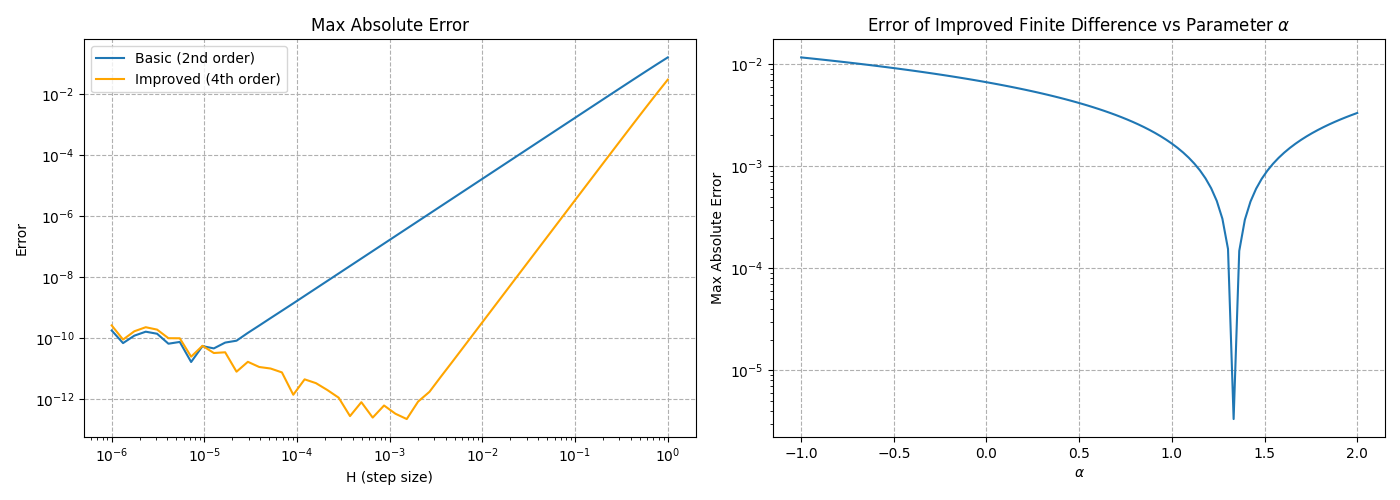
\includegraphics[scale=0.43]{img/finite-diff/finite-difference.png}
    \caption{Left pane: Approximation error for second-order and fourth-order schemes.
        For small values of $H$, round-off errors dominate.
        Right pane: Approximation error vs. $\alpha$ in the improved finite difference scheme ($H = 0.1$).
        Note that the scheme is fourth-order accurate only for $\alpha = 4/3$ (cusp in the graph).}
    \label{fig:finite-diff-accuracy}
\end{figure}

We can alternatively define the finite difference operators in terms of the delta function to get rid of the dependence on the differenced function. (Technically, the resulting quantities are functions rather than operators.)
Consider for example the two-point finite difference in \autoref{eq:two-point-central-diff}.
The definition can be generalized beyond mesh points by letting
\begin{equation*}
    D_j(\phi)(\mathbf{x}) = -\frac{\phi(\mathbf{x} + H \mathbf{e}_j)-\phi (\mathbf{x} - H \mathbf{e}_j)}{2H} = -\int \left[ \frac{\delta(\mathbf{x} + H\mathbf{e}_j - \mathbf{x}') - \delta(\mathbf{x} - H\mathbf{e}_j - \mathbf{x}')}{2H} \right]\phi(\mathbf{x}')d\mathbf{x}',
\end{equation*}
where $\mathbf{e}_j$ is the $j$-th standard basis vector.
This motivates us to define
\begin{equation}\label{eq:two-point-central-diff}
    D_j(\mathbf{x}) = \frac{\delta(\mathbf{x} + H\mathbf{e}_j - \mathbf{x}') - \delta(\mathbf{x} - H\mathbf{e}_j - \mathbf{x}')}{2H}
\end{equation}
and
\begin{equation}\label{eq:four-point-central-diff}
    D_j(\mathbf{x}) = \frac{\delta(\mathbf{x} + H\mathbf{e}_j - \mathbf{x}') - \delta(\mathbf{x} - H\mathbf{e}_j - \mathbf{x}')}{2H} + (1-\alpha)\frac{\delta(\mathbf{x} + 2H\mathbf{e}_j - \mathbf{x}') - \delta(\mathbf{x} - 2H\mathbf{e}_j - \mathbf{x}')}{4H}
\end{equation}
as the two-point as four-point finite difference operators respectively.

If $\phi$ denotes the gravitational potential, then the field $\mathbf{g}$ is approximated at mesh point $\mathbf{x}_\mathbf{p}$ as
\begin{equation*}
    \mathbf{g}(\mathbf{x}_\mathbf{p}) = -\mathbf{D}(\phi)(\mathbf{x}_\mathbf{p}).
\end{equation*}

\subsection{Interpolation}
The value of the field strength $\mathbf{g}(\mathbf{x})$ at the position particle's position $\mathbf{x}$ is calculated by interpolating the values of $\mathbf{g}$ from the neighboring mesh-points.
Formally,
\begin{equation*}
    \mathbf{g}(\mathbf{x}) = \sum_\mathbf{p} W(\mathbf{x} - \mathbf{x}_\mathbf{p}) \mathbf{g}(\mathbf{x}_\mathbf{p}).
\end{equation*}
In practice, there is no need to sum over all mesh points.
Instead, we use an algorithm analogous to \autoref{alg:density-assignment} to only include the cells with non-zero contribution to the sum.
The method is illustrated in \autoref{alg:interpolation}.
\begin{algorithm}
    \caption{Field strength interpolation}\label{alg:interpolation}
    \begin{algorithmic}[1]
        \ForAll {particle $i$}
        \ForAll {cell $\mathbf{q}$ in $\mathcal{C}_S(\mathbf{x}_i)$}
        \State $\mathbf{g}(\mathbf{x}_i) \gets \sum_\mathbf{q} W(\mathbf{x}_i - \mathbf{x}_\mathbf{q}) \mathbf{g}(\mathbf{x}_\mathbf{q})$
        \EndFor
        \EndFor
    \end{algorithmic}
\end{algorithm}
It is important to note that in order to retain correct physical behavior, the interpolation and mass assignment schemes must use the same shape to represent the particles.
The procedure in \autoref{alg:interpolation} is trivially parallelized by converting the sequential loop into a parallel one.

The procedures of density assignment and interpolation presented in \autoref{alg:density-assignment} and \autoref{alg:interpolation} are high level description.
More concrete formulations suitable for direct use in an implementation are given in \cite{Hockney1988} and \cite{Kravtsov2002PM}.

\subsection{Code units}
Implementation of the PM (and \PThreeM{}) methods can be simplified by switching to a system of dimensionless units, often called \textit{code units}.
The natural units of time and length in a PM simulation are $H$ and $DT$, respectively.
Hence, length in a PM code is conveniently expressed in terms of multiples of $H$, and similarly time intervals are given as a multiple of $DT$, i.e. the conversion relations are
\begin{equation*}
    x' = \frac{x}{H} \quad \text{and} \quad t' = \frac{t}{DT}.
\end{equation*}
From there, it follows that
\begin{equation*}
    v' = \frac{DT}{H}v \quad \text{and} \quad a' = \frac{DT^2}{H}a.
\end{equation*}
The expected relation $\mathbf{g}' = -\nabla' \phi'$ leads to the definition $\phi' = (DT^2 / H^2)\phi$.
By stipulating that we have $\nabla'^2\phi = \rho'$, we get $\rho' = DT^2 \cdot 4\pi G\rho$, $m' = (DT^2\cdot 4\pi G / H^3) m$, and $G' = 1/(4\pi)$.

\subsection{Properties of the calculated field}
The accuracy of a simulation using a PM code depends on a variety of factors.
The user can decide to use any combination of the following elements that parameterize the program:
\begin{itemize}
    \item mass assignment and interpolation scheme: NGP, CIC, TSC, or possibly any other scheme from the infinite hierarchy described in \autoref{subsec:mass-assignment};
    \item convolution with the Green's function derived from the discretized Laplacian (\autoref{eq:dft-transformed-phi}) or the ``poor man's solver'' (\autoref{eq:poor-mans-poisson-solver});
    \item gradient approximation: two-point or four-point finite difference;
    \item grid resolution: number of meshpoints in each dimension.
\end{itemize}
In this subsection we analyze these choices have in from two different angles.
We first focus on the properties of the field produced by a single source which gives insight into the behavior of the simulation on the basis of pair-wise interparticle interaction.
Then, we analyze the global error in force calculation by comparing the PM-calculated forces acting on all particles in a typical simulation with forces produced by the PP method.

\subsubsection{Local picture}
The field produced by the PM method is neither homogenous nor isotropic.
Anisotropy can be observed by measuring the field generated by a particle in two different directions.
In \autoref{fig:pm-field-properties}, the field strength calculated using the PM method (with the Green's function derived from discrete Laplacian) due to a single source at $x = H$ is shown in two variants: when measured along the $x$-axis (blue line) and the $x=y$ line (orange line).
The difference between these two graphs illustrates anisotropy of the calculated field.
The figure also shows the field strength measured along the $x$-axis when the source was shifted by $H/2$ in the $-x$ direction (green line).
Its deviation from the case when the source was placed at $x=H$ (the blue graph) exemplifies inhomogeneity of the field computed using the PM method.
\begin{figure}[htp]
    \centering
    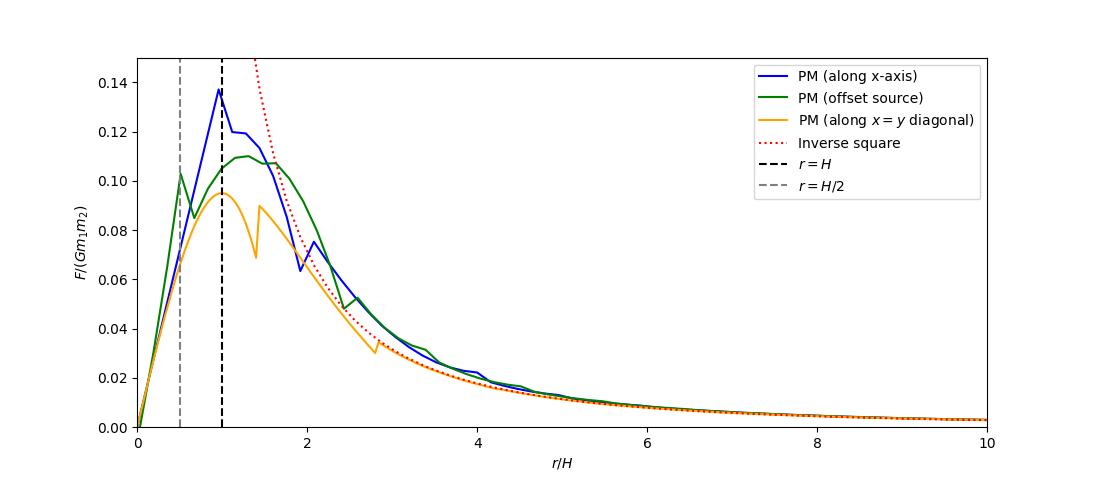
\includegraphics[scale=0.55]{img/pm/pm-field-combined.png}
    \caption{Anisotropy and inhomogeneity of the field as calculated by the PM method (TSC assignment, second order finite difference).}
    \label{fig:pm-field-properties}
\end{figure}
As expected, the PM-calculated approximation gets better with increasing distance from the source;
the inverse-square law is reproduced accurately for $r \gtrsim 4H$.

The single-source case analysis can be extended by considering the effect of choice of finite difference and mass assignment schemes on the relative error between the actual and approximated field strength.
\autoref{fig:pm-combined} shows a comparison of (a) the relative error as a function of distance from the source for PM with second-order and fourth-order finite differences, and (b) the field strength computed using different mass assignment schemes discussed in \autoref{subsec:mass-assignment}.
\begin{figure}[htp]
    \centering
    \begin{subfigure}[t]{0.48\textwidth}
        \centering
        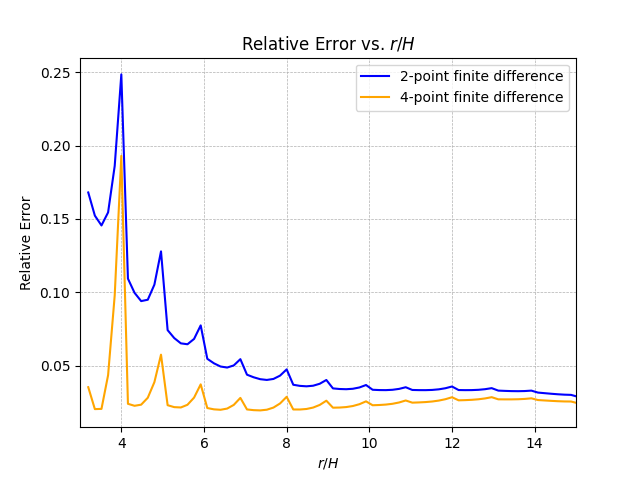
\includegraphics[width=\linewidth]{img/pm/pm-finite-diff-err.png}
        \caption{Relative error of field strength approximation in different PM variants.}
        \label{fig:pm-finite-diff-err}
    \end{subfigure}
    \hfill
    \begin{subfigure}[t]{0.48\textwidth}
        \centering
        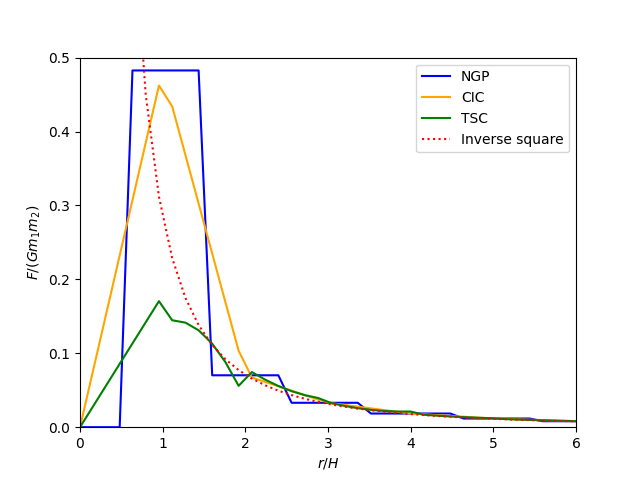
\includegraphics[width=\linewidth]{img/pm/pm-mass-assignment.png}
        \caption{Field strength calculated with the PM method using different assignment schemes.}
        \label{fig:pm-mass-assignment-field-strength}
    \end{subfigure}
    \caption{Comparison of PM method performance. (a) Relative error due to finite difference accuracy. (b) Effect of mass assignment schemes on computed field strength (4-point finite difference).}
    \label{fig:pm-combined}
\end{figure}
The conclusion that can be drawn from \autoref{fig:pm-combined} is that, as expected, the TSC mass assignment scheme and the four-point finite difference yield best results.

The field produced by the PM method using the ``poor man's'' potential solver is similar to the variant employing the discretized Laplacian Green's function described above.
\begin{figure}[htp]
    \centering
    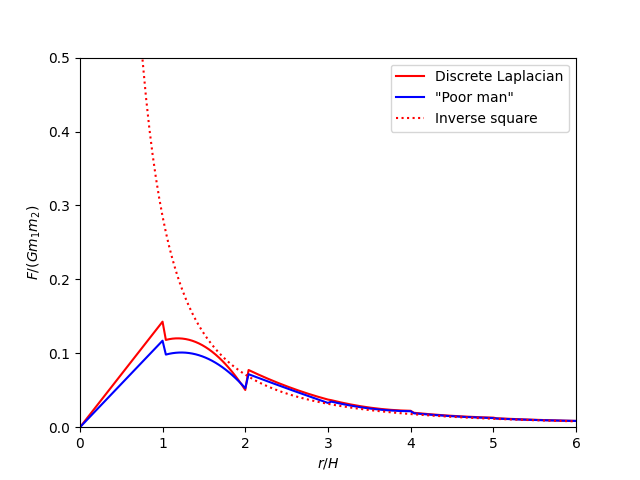
\includegraphics[scale=0.55]{img/poor-man-vs-laplacian.png}
    \caption{Field obtained potential calculated by the ``Poor man's Poisson solver'' vs. when using \autoref{eq:dft-transformed-phi}.}
    \label{fig:pm-poor-man-vs-laplacian}
\end{figure}

\subsubsection{Global picture}
To calculate the global approximation error of a PM simulation, we calculated the average of relative differences over all particles ($N=10{,}000$ in this case) between the forces produced by the PM method and the exact result obtained using the PP method.
More precisely, we the error was defined as
\begin{equation}\label{eq:force-avg-relative-err}
    \frac{1}{N}\sum_{i} \frac{|\mathbf{F}_i^\text{BH} - \mathbf{F}_i^\text{PP}|}{|\mathbf{F}_i^\text{PP}|}.
\end{equation}
The result, for different grid resolutions, is shown in \autoref{fig:pm-global-err-lap} ( $30 \leq N_g \leq 70$).
For the purposes of this test, the particle positions were generated according to the uniformly decreasing density disk model.
\begin{figure}[htp]
    \centering
    \begin{subfigure}[t]{0.48\textwidth}
        \centering
        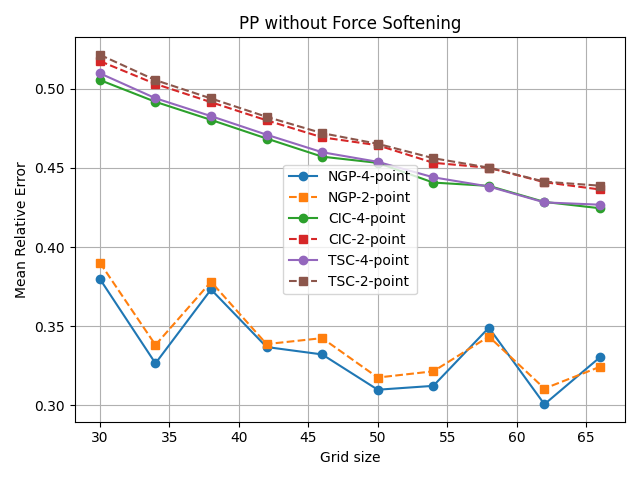
\includegraphics[width=\linewidth]{img/pm-global-err.png}
        \caption{PP calculation without force softening.}
        \label{fig:pm-global-err-lap-no-soft}
    \end{subfigure}
    \hfill
    \begin{subfigure}[t]{0.48\textwidth}
        \centering
        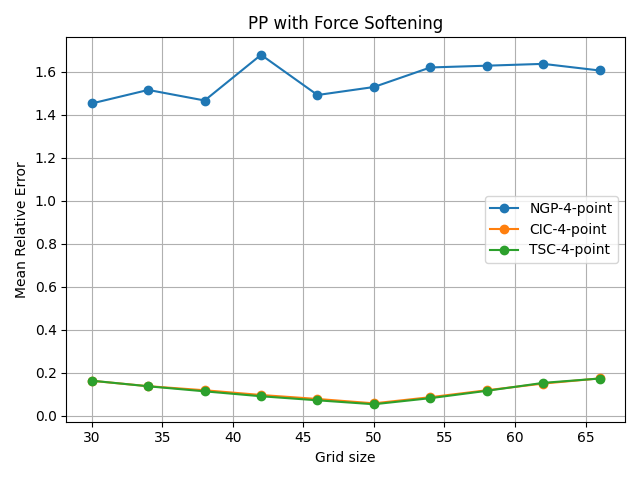
\includegraphics[width=\linewidth]{img/pm-global-err-soft.png}
        \caption{PP calculation with force softening.}
        \label{fig:pm-global-err-lap-soft}
    \end{subfigure}
    \caption{Average force approximation error in the PM method (discrete Laplacian solver).}
    \label{fig:pm-global-err-lap}
\end{figure}
As can be seen in \autoref{fig:pm-global-err-lap-no-soft}, for each of the assignment schemes, the error is minimized for the four-point difference, as expected.
A more surprising result is that the errors are seemingly greatest for the TSC assignment scheme.
This is easily explained by considering the graphs in \autoref{fig:pm-mass-assignment-field-strength}.
As can be seen there, the TSC assignment scheme gives raise to a force which accurately reproduces the inverse-square law force but at the same time it severely underestimates the force close to the source.
This behavior is expected since it stems from the mass of any individual particle being spread between multiple cells.
The CIC and NGP schemes on the other hand, do not reproduce the actual force with the same level of accuracy but the underestimation close the source is not as severe as in the case of the TSC scheme.
In some applications, for instance in the context of a galaxy simulation, this is a favorable feature of the TSC scheme.
The number of stars in a galaxy can be in the order of a trillion \cite{young2006andromeda}, whereas the number of particles in our tests is in the order of tens of thousands, giving an average of around $10^{12} / 10^{4} = 10^8$ of stars per particle.
As can be seen, it would be a serious mistake to model the force due to a single particle by the force due to a dimensionless point mass.
In such a case it is a standard practice to use a softened gravitational force instead of the one given in \autoref{eq:law-of-uni-grav} \cite{10.1046/j.1365-8711.2000.03316.x}.
By using the TSC scheme, force softening is automatically included in the calculation.
It can be argued that obtaining the smoothness properties enjoyed by the higher-order assignment schemes should be treated as tangential to softening the force.
It is for this reason, that Hockeney and Eastwood introduce the notion of \textit{force sharpening} as an additional step in the PM method in \cite{Hockney1988}.
In this modified version of the PM method, the Poisson equation takes the form
\begin{equation*}
    \nabla^2 \phi_p = \rho_p^*,
\end{equation*}
where $\rho^*_p$ is obtained from the density $\rho_p$ by solving the following system
\begin{equation*}
    1+\frac{\rho^*_{p+1} - 2\rho^*_p + \rho^*_{p-1}}{8}
    = \rho_p,
\end{equation*}
where $p$ indexes the mesh points.
In this work we do not investigate this matter further nor do we implement this modification in our program.

Now we return to the test whose results are presented in \autoref{fig:pm-global-err-lap}.
In the light of the above discussion, it is more reasonable to compare the quality of the results of the PM method with a \textit{softened gravitational force} defined in \cite{Zhang_2019} as
\begin{equation}\label{eq:softened-force}
    \mathbf{F}^\textrm{soft}_{ij} = -G\frac{m_i m_j}{(r_{ij}^2 + \epsilon^2)^{3/2}}\mathbf{r}_{ij}.
\end{equation}
The relative difference between the softened-forces and the PM-calculated ones is shown in \autoref{fig:pm-global-err-lap-soft}.
The \textit{softening length} $\epsilon$ was fixed at around $1H$ in the $64 \times 64 \times 32$ mesh configuration.
As the resolution of the mesh increases, the softening induced by the PM method becomes weaker so we should expect a minimum on the graph shown in \autoref{fig:pm-global-err-lap} corresponding to the point at which the PM-force starts to resemble the true inverse-square force more than the softened force.
This point in our test happens to be at around 50 meshpoints per dimension.

\subsection{Implementation}

\section{Particle-particle particle-mesh method}
The \PThreeM{} algorithm is a hybrid method:
Forces between distant particles are calculated using the PM method, whereas, for particles lying closely together, the PP method is used.
The total force applied to particle $i$ is
\begin{equation}\label{eq:p3m}
    \mathbf{F}_i^\text{SR} + \mathbf{F}_i = \sum_{j \neq i}(\mathbf{f}_{ij}^\text{tot} - \mathbf{R}_{ij}) + \mathbf{F}_i,
\end{equation}
where $\mathbf{F}_i \approx \sum_{j\neq i} \mathbf{R}_{ij}$ is the force computed using the PM method and $\mathbf{R}_{ij} = \mathbf{R}(\mathbf{x}_i - \mathbf{x}_j)$ is a prescribed \textit{reference force}.
The reference force is defined as the force between two particle-clouds, i.e. each particle is represented by a sphere with diameter $a$ and a given density profile.
The two examples of reference forces described in \cite{Hockney1988} are
\begin{equation*}
    R(r) =
    G m_1 m_2 \times\begin{cases}
        \frac{1}{35 a^2} (224 \xi - 224 \xi^3 + 70 \xi^4 + 48 \xi^5 - 21 \xi^6),                               & 0 \leq \xi \leq 1 \\
        \frac{1}{35 a^2} (12 / \xi^2 - 224 + 896 \xi - 840 \xi^2 + 224 \xi^3 + 70 \xi^4 - 48 \xi^5 + 7 \xi^6), & 1 < \xi \leq 2    \\
        \frac{1}{r^2},                                                                                         & \xi > 2
    \end{cases}
\end{equation*}
where $\xi = 2r/a$ for a sphere with uniformly decreasing density (shape $S_2$) and
\begin{equation}\label{eq:s1-reference-force}
    R(r) =
    G m_1 m_2 \times\begin{cases}
        \frac{1}{a^2} (8 r / a - 9 r^2 / a^2 + 2 r^4 / a^4), & r < a \\
        \frac{1}{r^2},
    \end{cases}
\end{equation}
for a solid sphere (shape $S_1$).
The reference force vector lies along the line joining the two bodies.

\subsection{Optimal Green's function}
As it is apparent from \autoref{eq:p3m}, the method's validity depends on how well the reference force is approximated by the mesh force.
The average deviation between the two forces can be minimized by a suitable choice of Green's function given (in $k$ space) by
\begin{equation}\label{eq:optimal-greens-func}
    \hat{\mathcal{G}}(\mathbf{k}) = \frac{\hat{\mathbf{D}}(\mathbf{k}) \cdot \sum_{\mathbf{n}}\hat{U}^2(\mathbf{k_\mathbf{n}}) \hat{\mathbf{R}}(\mathbf{k}_\mathbf{n})}{|\hat{\mathbf{D}}(\mathbf{k})|^2 \left[ \sum_{\mathbf{n}}\hat{U}^2(\mathbf{k}_\mathbf{n}) \right]^2}.
\end{equation}
The derivation is mathematically involved and is detailed in \cite{Hockney1988}.
We now proceed to examine the terms appearing in \autoref{eq:optimal-greens-func}.

\subsubsection{Finite difference operator}
The Fourier transform $\hat{\mathbf{D}}$ of the two-point finite difference operator defined in \autoref{eq:two-point-central-diff} has the components
\begin{align*}
    \hat{D}_j(\mathbf{k})
     & = \int D_j(\mathbf{x}) e^{-i\mathbf{k}\cdot \mathbf{x}} d\mathbf{x}                                                                                                                                      \\
     & = \frac{1}{2H}\left( \int \delta(\mathbf{x} + H\mathbf{e}_j)e^{-i \mathbf{k}\cdot \mathbf{x}} d\mathbf{x} - \int \delta(\mathbf{x} - H\mathbf{e}_j)e^{-i \mathbf{k}\cdot \mathbf{x}} d\mathbf{x} \right) \\
     & = \frac{1}{2H} (e^{ik_j H} - e^{-ik_j H})
    = \frac{i \sin(k_j H)}{H}.
\end{align*}
Similarly, for the four-point finite difference (\autoref{eq:four-point-central-diff}) we have
\begin{equation*}
    \hat{D}_j = \alpha\frac{i\sin k_j H}{H} + (1- \alpha)\frac{i\sin 2k_j H}{2H},
\end{equation*}
where $j=1,2,3$.

\subsubsection{Assignment function}
The quantity $\hat{U}$ is defined as $\hat{W}/V$.
For the mass assignment scheme hierarchy described in \autoref{subsec:mass-assignment} we have
\begin{equation*}
    \hat{U}(\mathbf{k}) = \left(\prod_{i=1}^{3}\frac{\sin(k_i H / 2)}{k_i H / 2}\right)^{p},
\end{equation*}
where $p=1,2,3,\dots$ with $p=1$ corresponding to NGP assignment, etc.
In particular, for the TSC assignment scheme, the \textit{alias sum}\footnote{
    To get the alias sums compatible with the DFT definition given in \autoref{eq:standard-dft}, one has to compute
    \begin{equation*}
        \sum_{\mathbf{n}} \tilde{U}^2(\mathbf{k}_\mathbf{n})
        \equiv \sum_\mathbf{n}\tilde{U}^2(\mathbf{k}+\mathbf{n}N)
        = \frac{1}{H}\sum_\mathbf{n}\hat{U}^2\left(\mathbf{k}\frac{2\pi}{NH}+\mathbf{n}\frac{2\pi}{H}\right)
    \end{equation*}
    instead.
}
\begin{equation*}
    \sum_{\mathbf{n}}\hat{U}^2(\mathbf{k}_\mathbf{n})
    \equiv \sum_{\mathbf{n}}\hat{U}^2\left(\mathbf{k} + \mathbf{n}\frac{2\pi}{H}\right)
\end{equation*}
can be rewritten as
\begin{align*}
    \sum_{\mathbf{n}} \hat{U}^2\left(\mathbf{k}+\mathbf{n}\frac{2\pi}{H}\right)
     & = \sum_{\mathbf{n}} \prod_{i=1}^{3} \left[ \frac{\sin(k_i H/2 + n_i\pi)}{k_i H/2 + n_i\pi} \right]^6 \\
     & = \prod_{i=1}^{3} \sum_{n_i} \left[ \frac{\sin(k_i H/2 + n_i \pi)}{k_i H/2 + n_i \pi} \right]^6      \\
     & = \prod_{i=1}^{3} \left[ \sin^6\left(\frac{k_i H}{2}\right)
        \sum_{n_i} \frac{1}{(k_i H/2 + n_i \pi)^6} \right]
\end{align*}
Using the the partial fractions expansion of the cotangent function \cite{aigner2018proofs},
\begin{equation*}
    \frac{(-1)^s}{s!}\frac{d^s}{dx^s}\cot x = \sum_{n=-\infty}^{\infty} \frac{1}{(x-n\pi)^{s+1}},
\end{equation*}
we can simplify the sum over $n_i$ to
\begin{equation*}
    \frac{-1}{5!} \frac{d^5}{dx^5}\cot\left( \frac{k_i H}{2} \right)
    = 1 - \sin^2\frac{k_i H}{2} + \frac{2}{15}\sin^4\frac{k_i H}{2}.
\end{equation*}
Hence,
\begin{equation*}
    \sum_{\mathbf{n}}\hat{U}_\text{TSC}^2(\mathbf{k}_\mathbf{n})
    = \prod_{i=1}^{3} \left(1 - \sin^2\frac{k_i H}{2} + \frac{2}{15}\sin^4\frac{k_i H}{2}\right).
\end{equation*}
Using the same approach, we can obtain similar results for the CIC and NGP schemes, namely
\begin{equation*}
    \sum_{\mathbf{n}}\hat{U}_\text{CIC}^2 = \frac{1}{3} \prod_{i=1}^{3} \left(1 + 2\cos^2\frac{k_i H}{2}\right)
    \quad \text{and} \quad
    \sum_{\mathbf{n}}\hat{U}_\text{NGP}^2 = 1.
\end{equation*}

\subsubsection{Reference force}
The quantity $\hat{\mathbf{R}}$, the transformed reference force, is related to the shape $S$ of the particle-cloud by
\begin{equation}\label{eq:reference-force-transform}
    \hat{\mathbf{R}}(\mathbf{k}) = \frac{i\mathbf{k}\hat{S}^2(k)}{k^2},
\end{equation}
where $k = |\mathbf{k}|$.
This can be shown by recalling that $\mathbf{R}(\mathbf{x}_i - \mathbf{x}_j)$ is the force applied to cloud $i$ due to cloud $j$.
Hence $\mathbf{R}(\mathbf{x})$ is the force on cloud centered at $\mathbf{x}$ due to a cloud at the origin.
The force acting on mass element $d\mathbf{x}' S(\mathbf{x}' - \mathbf{x})$ of the cloud centered at $\mathbf{x}$ is therefore
\begin{equation*}
    -G d\mathbf{x}'S(\mathbf{x}' - \mathbf{x}) \int d\mathbf{x}'' S(\mathbf{x}'')\frac{\mathbf{x}' - \mathbf{x}''}{|\mathbf{x}' - \mathbf{x}''|^3}
\end{equation*}
and the total force is
\begin{equation}\label{eq:reference-force-clouds}
    \mathbf{R}(\mathbf{x}) = -G \int d\mathbf{x}'S(\mathbf{x}' - \mathbf{x}) \int d\mathbf{x}'' S(\mathbf{x}'')\frac{\mathbf{x}' - \mathbf{x}''}{|\mathbf{x}' - \mathbf{x}''|^3}.
\end{equation}
The expression on the right-hand side of \autoref{eq:reference-force-clouds} is a double convolution, $\mathbf{R} = -S * (S * \mathbf{g})$, where $\mathbf{g}(\mathbf{x}) = \mathbf{x}/|\mathbf{x}|^3.$
The $x$-coordinate of $\mathbf{g}$ is $x/|\mathbf{x}|^3$ which coincides with $\partial h / \partial x$ for $h(\mathbf{x}) = -1/|\mathbf{x}|.$
The Fourier transform of $h$ is given in \cite{gelfand1964generalized} (p. 363):
\begin{equation*}
    \hat{h}(\mathbf{k}) = \frac{4\pi}{|\mathbf{k}|^2}.
\end{equation*}
The formula for the transform of a derivative yields
\begin{equation*}
    \hat{g}_x(\mathbf{k}) = \frac{4\pi i k_x}{|\mathbf{k}|^2}.
\end{equation*}
Applying the convolution theorem twice and factoring the constant $(-4\pi G)$ out of the Green's function in \autoref{eq:optimal-greens-func} leaves us with the desired \autoref{eq:reference-force-transform}.

Since the shapes $S$ are spherically symmetric, the calculation of $\hat{S}$ (appearing in \autoref{eq:reference-force-transform}) can be simplified.
The Fourier transform of $S$ is
\begin{equation*}
    \hat{S}(\mathbf{k}) = \int S(\mathbf{x}) e^{-i\mathbf{k} \cdot \mathbf{x}} d\mathbf{x}.
\end{equation*}
Observe that $\mathbf{k} \cdot \mathbf{x} = kr\cos\theta$, where $\theta$ is the angle between $\mathbf{k}$ and $\mathbf{x}$ and $r = |\mathbf{x}|$.
Since $S$ is invariant under rotations, $\theta$ can be chosen to be the angle between $\mathbf{x}$ and the $z$-axis.
Thus, the integral, rewritten in spherical coordinates becomes
\begin{equation*}
    \hat{S}(k) = \int_{0}^{2\pi}d\phi \int_{0}^{\pi} d\theta \int_{0}^{\infty}dr S(r)e^{-ikr\cos\theta}r^2\sin\theta
    = 2\pi \int_{0}^{\infty} r^2 dr \int_{0}^{\pi} d\theta e^{-ikr\cos\theta} \sin\theta.
\end{equation*}
The $\theta$-integral upon the substitution $-kr\cos\theta \to u$ becomes
\begin{equation*}
    \frac{1}{kr}\int_{-kr}^{kr} e^{iu} du
    = \frac{1}{kr} \int_{-kr}^{kr} (\cos u + i \sin u) du
    = \frac{2\sin kr}{kr}
\end{equation*}
and hence
\begin{equation*}
    \hat{S}(k) = 4\pi \int_{0}^{\infty} r^2 S(r)\frac{\sin kr}{kr}dr.
\end{equation*}

This integral, evaluated for the $S_1$ and $S_2$ shapes respectively, gives
\begin{equation*}
    \hat{S_1}(k) = \frac{3}{(ka/2)^3} \left(\sin\frac{ka}{2} - \frac{ka}{2} \cos\frac{ka}{2}\right)
\end{equation*}
and
\begin{equation*}
    \hat{S_2}(k) = \frac{12}{(ka/2)^4}\left(2 - 2\cos\frac{ka}{2}-\frac{ka}{2}\sin\frac{ka}{2}\right).
\end{equation*}

Finally, we note that the infinite sum in the numerator of \autoref{eq:optimal-greens-func} does not have a closed form but this does not pose a problem since the summand decays rapidly with $\mathbf{n}$ moving further away from zero.

The result of applying the optimal Green's function in \autoref{eq:poisson-fourier-product} is shown in \autoref{fig:reference-force-approx}.
\begin{figure}[htp]
    \centering
    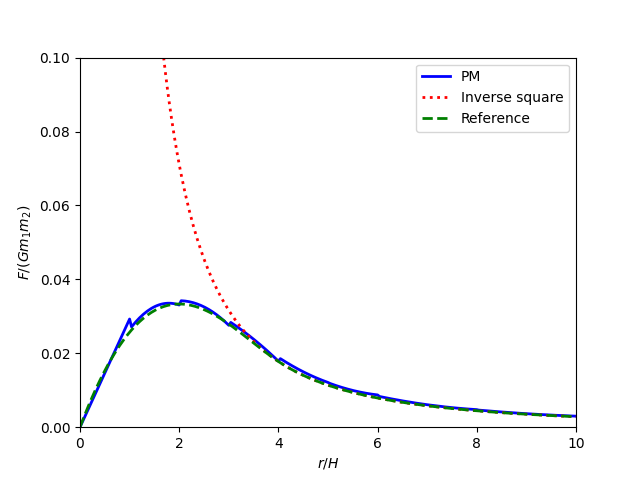
\includegraphics[scale=0.6]{img/optimal-green-force-4.png}
    \caption{Magnitude of the force between two masses.
        The mesh approximation to the reference force was calculated using the PM method with TSC assignment scheme, two-point finite difference, and Green's function optimal for the $S_1$ shape with diameter $a=4H$.
        The force resultant from the universal law of gravitation is also shown.}
    \label{fig:reference-force-approx}
\end{figure}
As can be seen in the figure, the PM force closely follows the reference force.
Moreover, for $r>a$, the reference force is identical to the inverse-square force.
It is also worth noting that the reference force (and its mesh approximation) approximates the inverse-square force accurately for $r$ slightly smaller than $a$.
For this reason $r_e$, the \textit{cutoff radius} designating the boundary of the region handled by the direct summation, can be chosen to be smaller than $a$ (e.g. $r_e = 0.7a$).
This can have a noticeable positive impact on performance.

\subsection{Identifying close pairs of particles}
In the \PThreeM{} method, in addition to the mesh used in the PM algorithm (the ``potential mesh''), a second mesh (the \textit{chaining mesh}) is used.
The chaining mesh is sparser than the potential mesh.
Its sole purpose is to partition the space into cells so that particles ``close'' to the ones in a given cell can be found efficiently.
In this context, two particles are considered to lie close to one another if their separation is less than the cutoff radius.

The number of chaining mesh cells in a single dimension is given by $M_i = \lfloor L_i / r_e \rfloor$, where $L_i$ is the side length of the computational box ($i=1,2,3$).
This implies that the side length of a chaining mesh cell is $HC_i = L_i / M_i \geq r_e$.
Thus, for every particle $i$ in a given cell $\mathbf{p}$, it is sufficient to search through the immediate neighborhood of $\mathbf{p}$ to find all the particles within the cutoff radius from $i$.

The chaining mesh can be implemented as a \textit{head-of-chain} (HOC) array, depicted in \autoref{fig:hoc}.
\begin{figure}[htp]
    \centering
    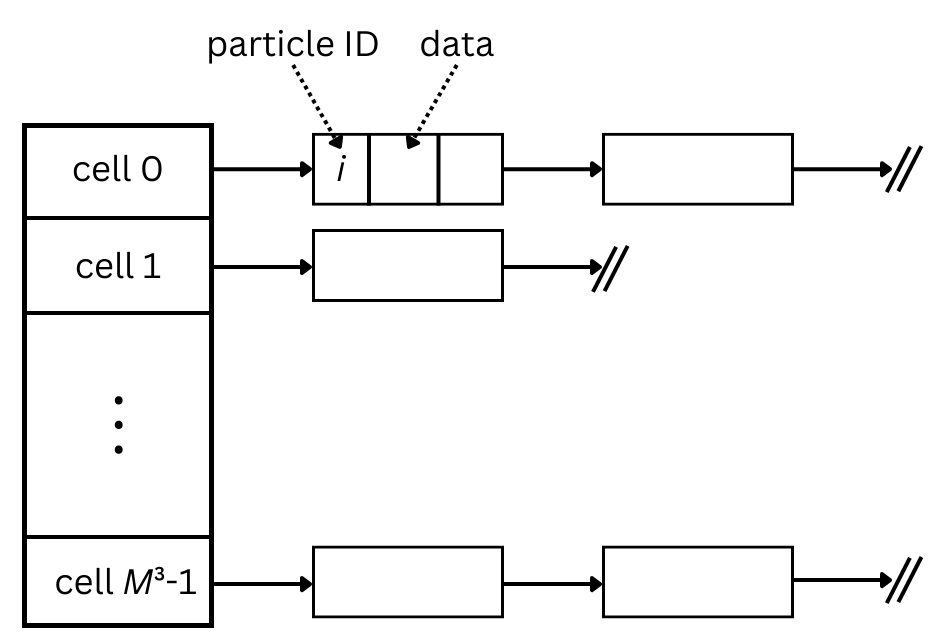
\includegraphics[scale=0.25]{img/hoc.png}
    \caption{Head-of-chain data structure used for mapping particles to their parent cells in the chaining mesh.
        Here $M_1=M_2=M_3 = M$.}
    \label{fig:hoc}
\end{figure}
The basic version of the HOC array is very cheap to build since the whole process is linear in the number of particles.
Hence, the array can be constructed anew at each time step.
Additional computational savings can be made by preallocating a memory pool large enough to store $N$ nodes of the linked lists and reusing it for the HOC array initialization.
Another noteworthy possible optimization is to sort the individual linked lists by the value of a particle coordinate of choice, say the $y$ coordinate.
This allows for an early return from the direct summation loop on the condition that $|y_i - y_j| > r_e$ while particle $i$ is sweeping through a cell containing particles $j$.

\subsection{Short-range correction}
The short-range correction, which takes place immediately after the mesh forces are found using the PM method, is at the heart of the \PThreeM{} algorithm.
Since it scales with a square of the number of particles in each neighborhood, further optimizations are highly desirable.

By Newton's 3rd law, $\mathbf{f}^\text{SR}_{ji} = -\mathbf{f}^\text{SR}_{ij}$, which allows us to do the calculation of the short-range inter-particle force for any pair $(i, j)$ of particles only once, leading to the reduction of the total running time by half.
In practice, the particle $i$ will update its total short-range force $\mathbf{F}^\text{SR}_i$ as well as the total short-range force $\mathbf{F}^\text{SR}_j$ of its neighbor $j$.
To avoid double-counting, the particle $i$ residing in cell $\mathbf{q}$ has to look for its neighbors in a subset $\mathcal{N}$ of the immediate neighborhood of $\mathbf{q}$.
More specifically, define
\begin{equation*}
    \mathcal{N}(\mathbf{q} = (q_1, q_2, q_3)) = \{(q_1+t, q_2-1,q_3+s), (q_1+s, q_2, q_3-1), (q_1-1,q_2,q_3) \;|\; s,t = -1,0,1 \}.
\end{equation*}
Thus $|\mathcal{N}| = 13$, which is half of the size of the immediate neighborhood.

The short-range correction part of the \PThreeM{} method is shown in \autoref{alg:short-range-correction}.
\begin{algorithm}
    \caption{Short-range correction}\label{alg:short-range-correction}
    \begin{algorithmic}[1]
        \ForAll {chaining cell $\mathbf{q}$}
        \ForAll {$\mathbf{q}_n \in \mathcal{N}(\mathbf{q}) \cup \{\mathbf{q}\}$}
        \ForAll {$i \in \text{HOC}(\mathbf{q})$}
        \ForAll {$j \in \text{HOC}(\mathbf{q}_n)$}
        \If {$|y_i - y_j| > r_e$}
        \Break
        \EndIf
        \State \Call{UpdateShortRange}{$i$, $j$, $\mathbf{q}$, $\mathbf{q}_n$}
        \EndFor
        \EndFor
        \EndFor
        \EndFor
    \end{algorithmic}
\end{algorithm}
The \textsc{UpdateShortRange} procedure is defined in \autoref{alg:update-short-range-forces}.
\begin{algorithm}
    \caption{Updating short-range forces}\label{alg:update-short-range-forces}
    \begin{algorithmic}[1]
        \Procedure{UpdateShortRange}{$i$, $j$, $\mathbf{q}$, $\mathbf{q}_n$}
        \If {$i = j$}
        \Return
        \EndIf
        \State $\mathbf{r}_{ij} \gets \mathbf{r}_i - \mathbf{r}_j$
        \If {$|\mathbf{r}_{ij}|^2 > r_e^2$}
        \Return
        \EndIf
        \State $r_{ij} \gets |\mathbf{r}_{ij}|$
        \State $\hat{\mathbf{r}}_{ij} \gets \mathbf{r}_{ij} / r_{ij}$
        \State $\mathbf{R}_{ij} \gets -m_i m_j R(r_{ij}) \hat{\mathbf{r}}_{ij}$
        \State $\mathbf{f}^\text{tot} \gets -G m_i m_j / r_{ij}^2 \hat{\mathbf{r}}_{ij}$
        \State $\mathbf{f}^\text{SR}_{ij} \gets \mathbf{f}^\text{tot} - \mathbf{R}_{ij}$
        \State $\mathbf{f}^\text{SR}_{ji} \gets -\mathbf{f}^\text{SR}_{ij}$
        \State $\mathbf{F}^\text{SR}_i \gets \mathbf{F}^\text{SR}_i + \mathbf{f}^\text{SR}_{ij}$
        \If {$\mathbf{q}_n \neq \mathbf{q}$} \Comment{Avoid double-counting in the parent cell}
        \State $\mathbf{F}^\text{SR}_j \gets \mathbf{F}^\text{SR}_j + \mathbf{f}^\text{SR}_{ji}$
        \EndIf
        \EndProcedure
    \end{algorithmic}
\end{algorithm}
As suggested in \cite{Hockney1988}, the computational burden of operations in lines 5-8 in \autoref{alg:update-short-range-forces} can be greatly reduced by storing the values of $f^\text{SR}(r) / r = (f^\text{tot}(r) - R(r)) / r$ in a lookup table $T$ at uniform intervals $\Delta^2$ of $[0, r_e^2]$ and interpolating.
The schematic depiction of the interpolation is shown in \autoref{fig:sr-force-val-interpolation}.
\begin{figure}[htp]
    \centering
    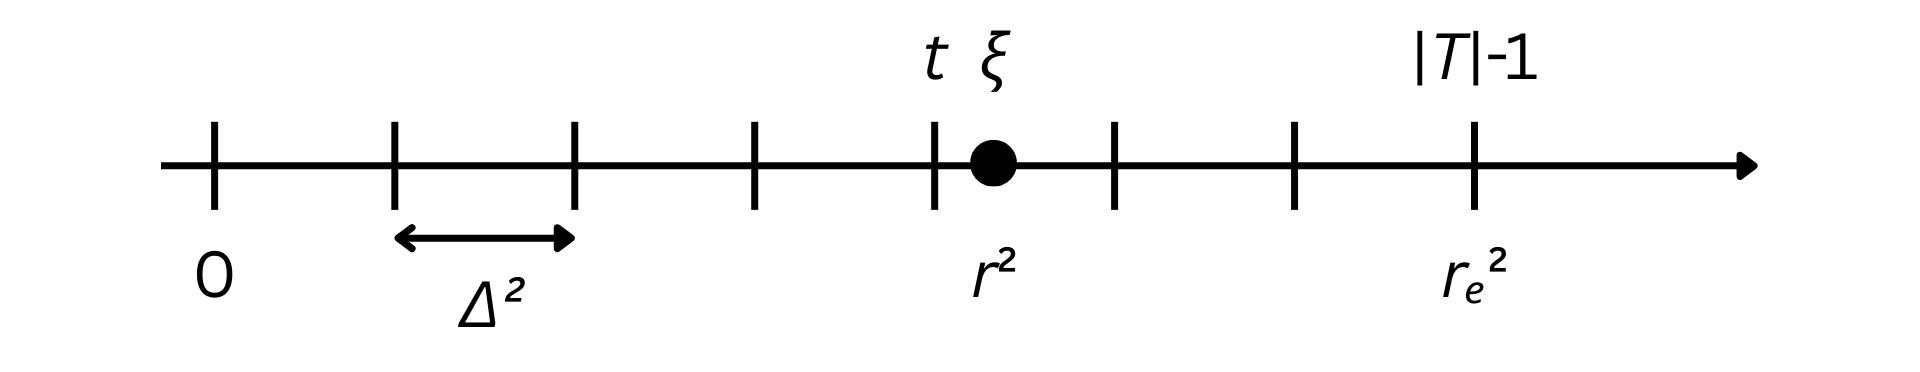
\includegraphics[scale=0.2]{img/interpolation.png}
    \caption{Interpolation of short-range force values.}
    \label{fig:sr-force-val-interpolation}
\end{figure}
If we define $\xi = r^2 / \Delta^2$ and $t=\lfloor \xi \rfloor$, then
\begin{equation*}
    \frac{f^\text{SR}(r)}{r} \approx T[t]\left(1 - (\xi - t)\right) + T[t+1](\xi - t)
    = T[t] + (\xi - t) (T[t+1] - T[t]).
\end{equation*}
The value $\mathbf{f}^\text{SR}_{ij}$ can then be obtained by multiplying the interpolated quantity $f^\text{SR}(r_{ij})/r_{ij}$ by $G m_i m_j \mathbf{r}_{ij}$, eliminating the use of the square root operations and reducing the total number of floating-point operations to just four.

The procedure outlined in\autoref{alg:short-range-correction} can be parallelized by splitting the work done in the outmost loop between some number of threads.
In doing so, extra care has to be taken to avoid data races.
A thread $t$ that is currently processing cell $\mathbf{p}$ and its neighbors (we say that $t$ is \textit{assigned} to $\mathbf{p}$) may ``clash'' with a different thread assigned to a nearby cell $\mathbf{q}$ (because possibly $\mathbf{p} \in \mathcal{N}(\mathbf{q})$).
However, by the construction of the set $\mathcal{N}$, it is possible to split the short-range force into 14 parts, each of which is accessed by only one thread.
For example, consider a particle $i$ in cell $\mathbf{p} = (p_1, p_2, p_3)$ (in other words, $\mathbf{p}$ is the parent cell of $i$).
If thread $t$ is currently assigned to this cell, $t$ will update the part of $\mathbf{F}^\text{SR}_i$ corresponding to updates of $i$ coming from within the same cell as the parent cell of $i$.
Possibly at the same time, thread $t'$ assigned to cell $\mathbf{q} = (p_1+1, p_2, p_3)$ will update a different part of $\mathbf{F}^\text{SR}_i$, i.e. the part corresponding to updates of $i$ coming from the cell ``to the right'' of the parent cell of $i$.
Since only one thread is responsible for updates to particle $i$ coming ``from the right,'' (or any other ``direction'') no data races can occur.
This approach has two drawbacks.
First, memory requirements increase significantly as memory for $13N$ additional three-dimensional vectors has to be used.
Second, there is no way to guarantee uniform work distribution among the threads.
\section{Barnes-Hut algorithm}
The idea behind Barnes-Hut algorithm differs substantially from previously described mesh-based methods.
The algorithm deals with gravitational forces directly instead of deriving them from the mesh-defined potential, as was the case with the PM and \PThreeM{} methods.
Significant reduction of time complexity, from quadratic to $O(N \log N)$, is achieved by approximating the potential due to ``far enough'' groups of particles by the initial terms of its multipole expansion \cite{trenti2008gravitationalnbodysimulations}.
The grouping of particles is hierarchical in nature and is thus best understood as a tree.
The entire set of particles comprises the top-level group, represented by the root of the tree;
the eight children of the root node are representative of groups of particles residing in each of the octants of the computational domain, etc.
The process of subdividing the space into eight smaller volumes at each node continues recursively until there is only one or zero particles left in a given volume.
Nodes which satisfy this condition are the leafs of tree and are sometimes called the \textit{external nodes}.
The remaining nodes, each of which has eight children, are called \textit{internal nodes}.

In the basic variant of the algorithm, the potential due to a group of particles is approximated using only the monopole term with respect to the center of mass of the group, i.e.
\begin{equation*}
    \phi_\text{mon}(r) = -\frac{GM}{r},
\end{equation*}
where $M$ is the group's total mass.
Since the potential is expanded about the center of mass, the dipole moment $\mathbf{p} = \sum_{i} m_i \mathbf{r}_i$ vanishes.
Hence, the next possible improvement comes from including the quadrupole term
\begin{equation*}
    \phi_\text{quad}(r) = -\frac{G}{2r^5} \mathbf{r} \cdot (\mathbf{Q} \mathbf{r}),
\end{equation*}
where $\mathbf{Q}$ is the quadrupole moment tensor defined as
\begin{equation*}
    Q_{ij} = \sum_{k} (3r_{ki}r_{kj} - 3r_k^2\delta_{ij})m_k.
\end{equation*}
In theory, we could keep on adding more terms to improve the quality of the approximation.
In our implementation however, we restrict ourselves to the quadrupole term.

\subsection{Building the tree}
The data structure that fits the description given in the introduction is called an \textit{octree}.
An internal node of the octree stores the COM vector, the total mass of the group it represents, and the quadrupole tensor, whereas an external node stores a reference to the actual particles (or is empty if no particle was found in its associated volume).
The recursive procedure of building the tree is shown in \autoref{alg:bh-tree-insert}.
\begin{algorithm}
    \caption{Insert a particle into the Barnes-Hut tree}\label{alg:bh-tree-insert}
    \begin{algorithmic}[1]
        \Function{Insert}{$n$, $p$}
        \If{$n$ is an internal node}
        \State Update $n.\textrm{COM}$ and total mass $n.M$ of $n$ with $p$
        \State \Call{Insert}{child of $n$ that should contain $p$, $p$}
        \ElsIf{$n$ is empty}
        \State Assign $p$ to $n$
        \Else \Comment{Occupied external node}
        \State Subdivide $n$ into child nodes
        \State Move existing particle $p'$ in $n$ into child that should contain $p'$
        \State Update center of mass and total mass of $n$ with $p$ and $p'$
        \State \Call{Insert}{child of $n$ that should contain $p$, $p$}
        \EndIf
        \EndFunction
    \end{algorithmic}
\end{algorithm}
The quadrupole moment tensor for each node is calculated once the whole tree is already built.
The recursive relation used in this calculation is given in \cite{hernquist1987performance} and reads
\begin{equation*}
    \mathbf{Q} = \sum_{\text{child }c} \mathbf{Q}_c + \sum_{\text{child }c} m_c(3 \mathbf{R}_c \otimes \mathbf{R}_c - R_c^2 \mathbf{I}),
\end{equation*}
where $\mathbf{R}_c = \mathbf{x}^\text{COM}_c - \mathbf{x}^\text{COM}$ is the displacement vector from the COM of child $c$ to the COM of the parent, $\mathbf{I}$ is the identity matrix, and $\otimes$ denotes the outer product.

\subsection{Acceleration calculation}
In the Barnes-Hut algorithm, the net acceleration of a particle $p$ is calculated by summing the contributions from single particles or groups of particles while traversing the tree.
The decision whether the acceleration can be approximated using the information stored in an internal node $n$ depends on the relative distance from $p$ to $n.\textrm{COM}$ (the center of mass of group represented by $n$).
The distance is relative to the \textit{width} $H$ of the node, i.e. the side length of the cubical volume encompassed by the node.
More concretely, the approximation takes place if $n.H / |n.\mathrm{COM} - p.\mathbf{x}| < \theta$, where $\theta$ is the so-called \textit{opening angle}.
In the extreme case when $\theta$ is set to zero, no approximations take place, and the algorithm reduces to the PP method.
The procedure described above is illustrated in \autoref{alg:bh-find-force}.
\begin{algorithm}
    \caption{Compute gravitational force on a particle using Barnes-Hut approximation}
    \label{alg:bh-find-force}
    \begin{algorithmic}[1]
        \Function{FindAcceleration}{$n$, $p$, $\theta$}
        \If{$n$ is an external node}
        \If{$n$ contains a particle $q \neq p$}
        \State $p.\mathbf{a} \gets p.\mathbf{a} + \Call{GravitySoft}{q.\mathbf{x}, q.m, p.\mathbf{x}} / p.\text{mass}$
        \EndIf
        \State \Return
        \EndIf
        \If{$n.H / |n.\text{COM} - p.\mathbf{x}| < \theta$}
        \State $p.\mathbf{a} \gets p.\mathbf{a} + \Call{Gravity}{n.\mathrm{COM}, n.M, p.\mathbf{x}}$
        \State \Return
        \EndIf
        \ForAll{child $n_c$ of $n$}
        \State \Call{FindAcceleration}{$n_c$, $p$, $\theta$}
        \EndFor
        \EndFunction
    \end{algorithmic}
\end{algorithm}
In the implementation, the \textsc{GravitySoft} function calculates the gravitational force softened by $\epsilon$, i.e. it returns the value given by \autoref{eq:softened-force}.
The pairwise potential energy associated with this force is given by
\begin{equation}\label{eq:pe-soft}
    \Phi_{ij}^\textrm{soft} = - \frac{G m_i m_j}{\sqrt{r_{ij}^2 + \epsilon^2}}.
\end{equation}
The \textsc{Gravity} function returns the approximation (up to the quadrupole term) of the acceleration due to a group of particles represented by a given node, i.e.
\begin{equation*}
    \mathbf{a} = -GM \frac{\mathbf{r}}{r^3} + \frac{G}{r^5}\mathbf{Q}\mathbf{r} - \frac{5G}{2}(\mathbf{r} \cdot (\mathbf{Q} \mathbf{r})) \frac{\mathbf{r}}{r^7}
\end{equation*}
(see \cite{hernquist1987performance}).

One possible way to quantify the quality of approximation for a given value of $\theta$ is to consider the relative error of calculated force.
We set the same initial conditions of the system for both the PP direct summation method and the Barnes-Hut algorithm, compute the deviation of Barnes-Hut forces from PP forces acting on each particle, and take the average over all particles.
In other words, the error calculated is given by the \autoref{eq:force-avg-relative-err}.
The dependence of the error on the opening angle $\theta$ and the corresponding execution time are shown in \autoref{fig:bh-analysis}.
The figure includes plots for two cases: when only the monopole term is used in the Barnes-Hut approximation, and when both the monopole and quadrupole terms are included.
As can be seen, the quadrupole-based algorithm exhibits significantly improved error scaling with increasing $\theta$.
Naturally, this raises the question of the additional computational cost incurred by the inclusion of the quadrupole term.
Our tests showed that this impact is minimal.
The results (for $N = 10{,}000$ particles and $0 \leq \theta \leq 2$) support this observation.
\begin{figure}[htp]
    \centering
    \begin{subfigure}[b]{0.47\textwidth}
        \centering
        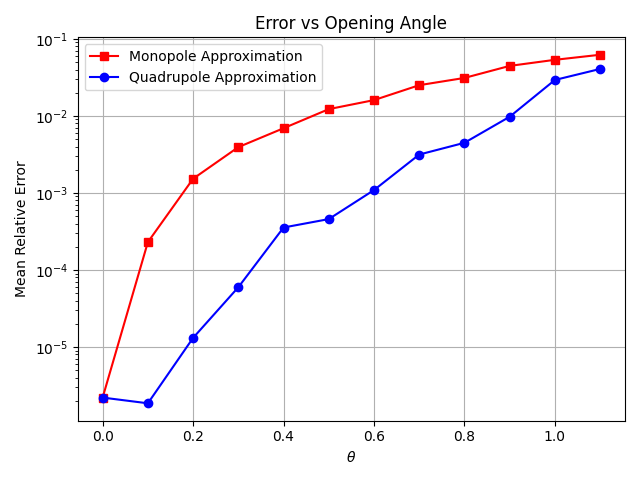
\includegraphics[width=\textwidth]{img/error-vs-theta.png}
        \caption{Force approximation error.}
        \label{fig:bh-force-error}
    \end{subfigure}
    \hfill
    \begin{subfigure}[b]{0.47\textwidth}
        \centering
        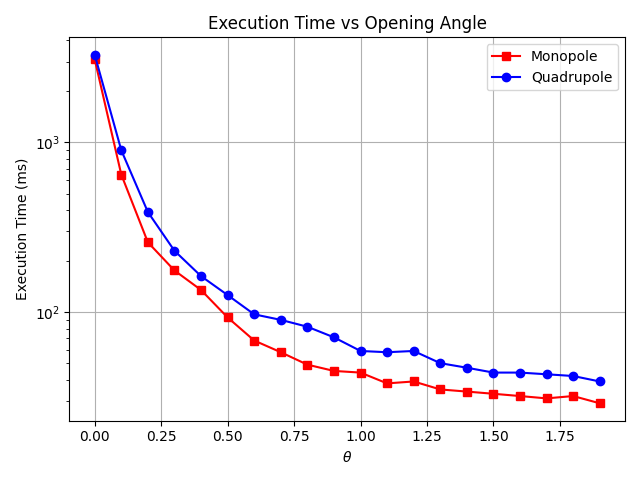
\includegraphics[width=\textwidth]{img/bh-time.png}
        \caption{Execution time.}
        \label{fig:bh-time}
    \end{subfigure}
    \caption{Comparison of error and execution time in the Barnes-Hut algorithm using monopole and quadrupole approximations.}
    \label{fig:bh-analysis}
\end{figure}
Both tests described above were conducted on a uniform disk particle distribution.

We note that direct calculation of total potential energy is infeasible as $O(N^2)$ operations would be required.
Instead, we use an approximation based on the values stored in the tree.
The approximate value of the potential energy is accumulated for each particle using a procedure analogous to force calculation.
Indeed, the only difference between the two is the replacement of gravitational force calculation in \autoref{alg:bh-find-force} with potential energy calculation according to \autoref{eq:pe-soft}.

It is also noteworthy that the procedure outlined in \autoref{alg:bh-find-force} is embarrassingly parallel.
In our CPU implementation, the workload is split between an arbitrary number of threads on particle-by-particle basis.
\section{Time integration}
In the previous sections we described various methods of calculating forces applied to particles in the simulation.
Once these forces are found, the evolution of the system in time can be tracked by integrating Newton's 2nd law of motion,
\begin{equation}\label{eq:newtons-second}
    \ddot{\mathbf{x}}_i = \frac{\mathbf{F}_i}{m_i}.
\end{equation}

\subsection{Euler's method}
Possibly, the simplest numerical method that could be used is Euler's method described by the update rules
\begin{equation}\label{eq:eulers-method}
    \begin{aligned}
        \mathbf{v}_i^{(k+1)} & = \mathbf{v}_i^{(k)} + DT \frac{\mathbf{F}^{(k+1)}_i}{m_i}, \\
        \mathbf{x}_i^{(k+1)} & = \mathbf{x}_i^{(k)} + DT \mathbf{v}_i^{(k)}.
    \end{aligned}
\end{equation}
The method defined in \autoref{eq:eulers-method} is not suitable for physical simulations, however.
Its shortcomings are best illustrated by an example of an undamped pendulum of length $l$ in gravitational field of magnitude $g$.
Although it is a simple system, it illustrates the numerical challenges faced in gravitational simulations over long timescales, particularly the issue of energy preservation.

The motion of the pendulum is governed by the differential equation
\begin{equation*}
    \ddot{\theta} = -\frac{g}{l}\sin\theta,
\end{equation*}
and its kinetic and potential energy are given by $KE = (1/2)ml^2\dot{\theta}$ and $PE = -mgl\cos\theta$ respectively.
\begin{figure}[htp]
    \centering
    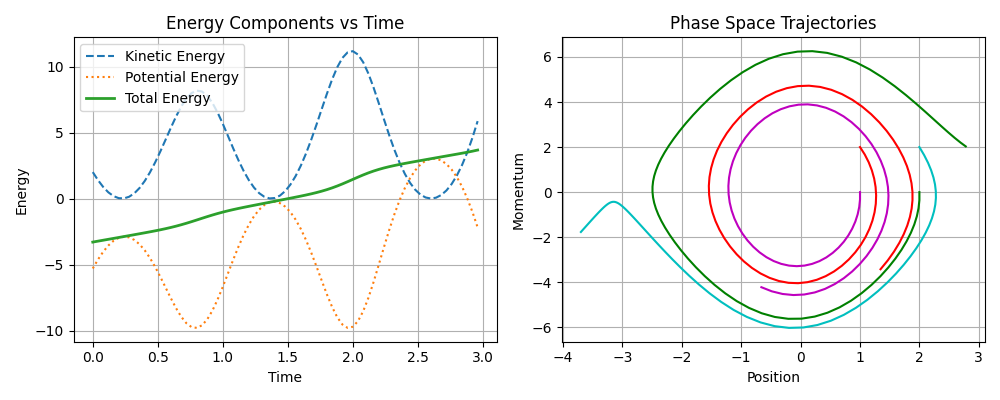
\includegraphics[scale=0.6]{img/integrators/euler-pendulum.png}
    \caption{Behavior of Euler's method: lack of conservation of energy and phase space trajectories spiraling out.}
    \label{fig:euler-integrator}
\end{figure}
As shown in \autoref{fig:euler-integrator}, Euler's method fails to conserve total energy $PE + KE$ and produces trajectories in phase space that are not closed, contrary to expectations for periodic systems.
Additionally, the evolution of an area element in phase space violates Liouville's theorem, as described in \cite{taylor2005classical}, making the method unsuitable for long-term physical simulations (see \autoref{fig:area-euler-vs-leapfrog}).
\begin{figure}[htp]
    \centering
    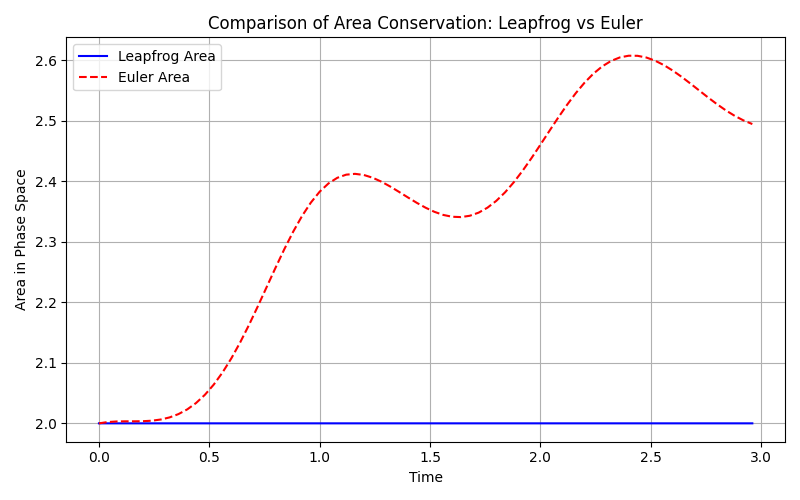
\includegraphics[scale=0.4]{img/integrators/area-leap-vs-euler.png}
    \caption{Area in phase space over time. Violation of Liouville's theorem by Euler's method.}
    \label{fig:area-euler-vs-leapfrog}
\end{figure}

\subsection{Leapfrog algorithm}
The leapfrog algorithm, given by the update rule \cite{young_leapfrog_2019}
\begin{equation}\label{eq:leapfrog}
    \begin{aligned}
        \mathbf{v}_{i}^{(1/2)} & = \mathbf{v}_i^{(0)} + \frac{1}{2}DT \frac{\mathbf{F}_i^{(0)}}{ m_i^{(0)}}, \\
        \mathbf{x}_i^{(k+1)}   & = \mathbf{x}_i^{(k)} + DT \mathbf{v}_i^{(k+1/2)},                           \\
        \mathbf{v}_i^{(k+3/2)} & = \mathbf{v}_i^{(k+1/2)} + DT \frac{ \mathbf{F}_i^{(k+1)}}{m_i}.
    \end{aligned}
\end{equation}
is the preferred way of integrating \autoref{eq:newtons-second}.
When applied to the same pendulum system, it conserves energy much more faithfully and preserves the area in phase space, consistent with Liouville's theorem (see \autoref{fig:leapfrog-integrator} and \autoref{fig:area-euler-vs-leapfrog}).
\begin{figure}[htp]
    \centering
    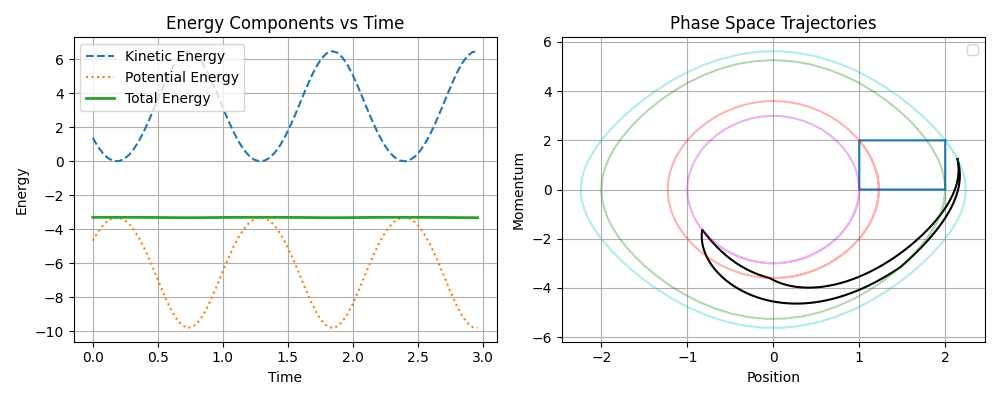
\includegraphics[scale=0.6]{img/integrators/leapfrog-pendulum.png}
    \caption{Behavior of the leapfrog algorithm: conservation of energy and phase space trajectories forming closed loops.
        Evolution of an area element in phase space is shown on the right-hand side: blue rectangle -- initial conditions for many copies of the system; black distorted quadrilateral -- their state by the end of the simulation.}
    \label{fig:leapfrog-integrator}
\end{figure}
Given its simplicity and excellent long-term energy behavior, we adopt the leapfrog algorithm to integrate Newton's equations in our program.
\section{Galaxy model}
The model of a galaxy used as a test bed for the implementation is a simple one.
The galaxy is assumed to be composed of only two parts: a thin disk and a central bulge.
The disk comprises a number of particles, each representing some number of stars.
The central bulge is simulated as a fixed external gravitational field.

\subsection{Disk}
The disk particles are sampled from a radial distribution
\begin{equation*}
    p(r) = \frac{3}{\pi R_D^2}\left(1 - \frac{r}{R_D}\right),
\end{equation*}
where $R_D$ is the radius of the disk and $r \leq R_D$.
The cumulative distribution function is therefore
\begin{equation*}
    F(r, \phi) = \int_{0}^{\phi}\int_{0}^{r} p(r') r'dr'd\phi' = \frac{\phi}{2\pi R_D^3}(3R_D r^2-2r^3)
\end{equation*}
and the marginal CDFs are
\begin{equation*}
    F_R(r) = F(r, 2\pi) = \frac{1}{R_D^3}(3R_D r^2-2r^3) \quad \text{and} \quad F_\Phi(\phi) = F(R_D, \phi) = \frac{\phi}{2\pi}.
\end{equation*}
Now we use inverse transform sampling to generate initial positions $(r, \phi)$ for the particles, i.e. $\phi = 2\pi u$ and $r$ is given implicitly by $h(r) \equiv 2r^3 - 3R_D r^2 + uR_D^3 = 0$ with $u \sim U(0, 1)$.
Straightforward calculation shows that $dh/dr < 0$ for $0 < r < R_D$ and $h(0)h(R_D) < 0$ implying that $h$ has exactly one zero between 0 and $R_D$ (which can be found for example using Newton's method).

Strength of the gravitational field $\mathbf{g}$ at point $\mathbf{x}_0$ is
\begin{equation*}
    \mathbf{g}_D = G \int_{0}^{2\pi}\int_{0}^{R_D} \sigma(r) \frac{\mathbf{x} - \mathbf{x}_0}{|\mathbf{x} - \mathbf{x}_0|^3}r dr d\phi,
\end{equation*}
where $\sigma(r) = \sigma_0(1 - r/R_D)$ describes the density profile of the disk for $r \leq R_D$.
If $M_D$ is the total mass of the disk, then $\sigma_0 = 3M_D / (\pi R_D^2)$.
By symmetry, the point $\mathbf{x}_0$ may be chosen to lie on the $x$-axis, i.e. $\mathbf{x}_0 = (-x_0, 0)$, so that $\mathbf{x} - \mathbf{x}_0 = (x_0 + r\cos\phi, r\sin\phi)$.
Letting $\bar{r} = r/R_D$ and $\bar{x}_0 = x_0 / R_D$, the integral becomes
\begin{equation*}
    \mathbf{g}_D = G\sigma_0 \int_{0}^{2\pi} \int_{0}^{1} (1 - \bar{r}) \frac{(\bar{x}_0 + \bar{r}\cos\phi, \bar{r}\sin\phi)}{|(\bar{x}_0 + \bar{r}\cos\phi, \bar{r}\sin\phi)|^3}\bar{r} d\bar{r} d\phi.
\end{equation*}
By symmetry $g_{D,y} = 0$ and thus the radial component of the field $\mathbf{g}_D$ at distance $R\bar{x}_0$ from the center is
\begin{equation}\label{eq:gx-disk}
    g_{D,r} = -G\sigma_0 \int_{0}^{2\pi} \int_{0}^{1} (1 - \bar{r})\frac{\bar{x}_0 + \bar{r}\cos\phi}{(\bar{x}_0^2+\bar{r}^2+2\bar{x}_0\bar{r}\cos\phi)^{3/2}}\bar{r}d\bar{r}d\phi.
\end{equation}
If the disk had constant density, $\mathbf{g}_D$ could be expressed in terms of elliptic integrals \cite{Weiss2018}.
However, to the best of the author's knowledge, the integral in \autoref{eq:gx-disk} cannot be further simplified.
For this reason, a crude approximation with a quadratic function is used: $g_{D,r} \approx a(r - h)^2 + k$, where the values $k=2.5$ and $h=0.66$ (the maximum of $g_{D,r}$ and the argument thereof) were estimated based on the graph of $g_{D,r}$ (see \autoref{fig:radial-strength-disk}).
The value of $a = -k/h^2$ can be found by setting $g_{D,r}(0) = 0$ in the approximate formula.
\begin{figure}[htp]
    \centering
    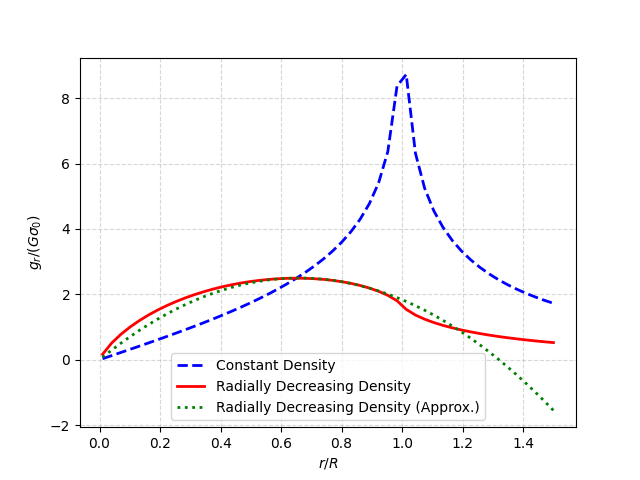
\includegraphics[scale=0.6]{img/disk-field.png}
    \caption{Magnitude of the radial component of the field strength due to a disk.
        The peak at $r=R$ for the constant density disk is in fact infinite.}
    \label{fig:radial-strength-disk}
\end{figure}

\subsection{Central bulge}
The density profile of the central bulge is analogous to the one used for the disk, save for the fact it is 3-dimensional, i.e.
\begin{equation*}
    \rho(r) =
    \begin{cases}
        \rho_0\left(1 - \frac{r}{R_B}\right), & r \leq R_B        \\
        0,                                    & \text{otherwise},
    \end{cases}
\end{equation*}
where $R_B$ is the radius of the bulge.
If we let $M_B$ be the mass of the bulge, then $\rho_0 = 3M_B / (\pi R_B^3)$.
Application of Gauss's law shows that we have
\begin{equation*}
    g_{B,r} = -G M_B \times
    \begin{cases}
        \frac{r}{R_B^3}r\left(4 - \frac{3r}{R_B}\right), & r \leq R_B        \\
        \frac{1}{r^2},                                   & \text{otherwise}.
    \end{cases}
\end{equation*}

\subsection{Initial conditions}
The total field $\mathbf{g} = \mathbf{g}_D + \mathbf{g}_B$ is used to find initial velocities for the particles with initial positions $(x, y, 0)$.
The formula for the centripetal force yields
\begin{equation*}
    \frac{v^2}{r} = -g_r
\end{equation*}
and thus
\begin{equation*}
    \mathbf{v} = \left(-v \frac{y}{r}, v\frac{x}{r}, 0\right)
\end{equation*}
with $v = \sqrt{- r g_r}$
for counter-clockwise rotation.

\section{Results}
The parameters used in the simulation of a spiral galaxy are shown in \autoref{tab:galaxy-parameters}.
\begin{table}[htp]
    \centering
    \begin{tabular}{|l|c|}
        \hline
        \textbf{Parameter}      & \textbf{Value}           \\
        \hline
        Halo radius             & 3 kpc                    \\
        Halo mass               & $60 \times 10^9 M_\odot$ \\
        Disk radius             & 15 kpc                   \\
        Disk mass               & $15 \times 10^9 M_\odot$ \\
        Disk thickness          & 0.3 kpc                  \\
        Disk density profile    & Uniformly decreasing     \\
        Mass assignment scheme  & TSC                      \\
        Finite difference       & Two-point                \\
        Time integration method & Leapfrog                 \\
        \hline
    \end{tabular}
    \caption{Galaxy model parameters used in the simulation.}
    \label{tab:galaxy-parameters}
\end{table}
The galaxy is simulated as an isolated system, however, in deriving \autoref{eq:poisson-fourier-product}, periodic boundary conditions were assumed.
The simplest way (and the one used) to obtain a free-space solution from the PM method is to extend the computational domain twice in every dimension and fill the space unused in mass distribution with zeros.
The total size of the potential mesh used was $128 \times 128 \times 64$ with the region of interest occupying a box of size $60\, \text{kpc}\times 60\, \text{kpc}\times 30\, \text{kpc}$ located in a $64 \times 64 \times 32$ octant of the mesh.

\subsection{Particle-mesh method}
In the PM method, $N=50,000$ particles were used.
Cell size $H$ and time-step length were set to $60/64=0.9375$ kpc, and 1 Myr respectively.
The system's evolution over 200 Myr is shown in \autoref{fig:spiral-galaxy-evolution-pm}.

\begin{figure}[htp]
    \centering
    \begin{subfigure}[b]{0.45\textwidth}
        \centering
        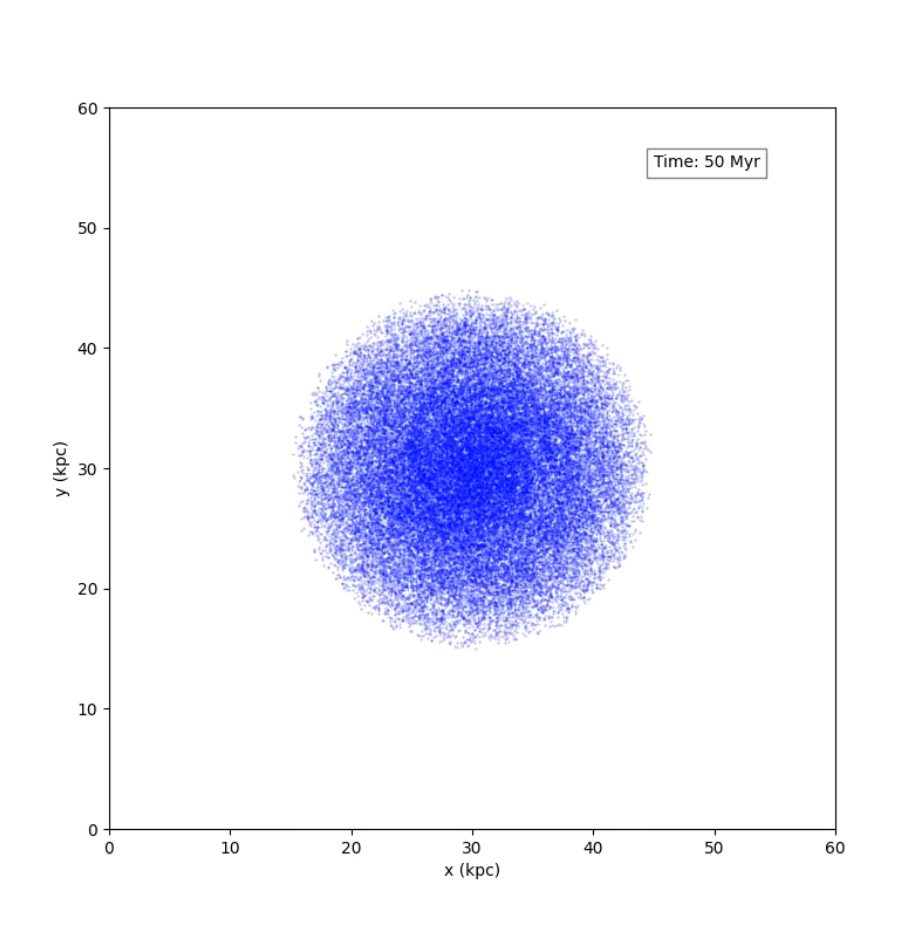
\includegraphics[width=\textwidth]{img/pm/50myr.png}
        \caption{$t=50\,\text{Myr}$}
        \label{fig:spiral-galaxy-evolution-pm-sub1}
    \end{subfigure}
    \hfill
    \begin{subfigure}[b]{0.45\textwidth}
        \centering
        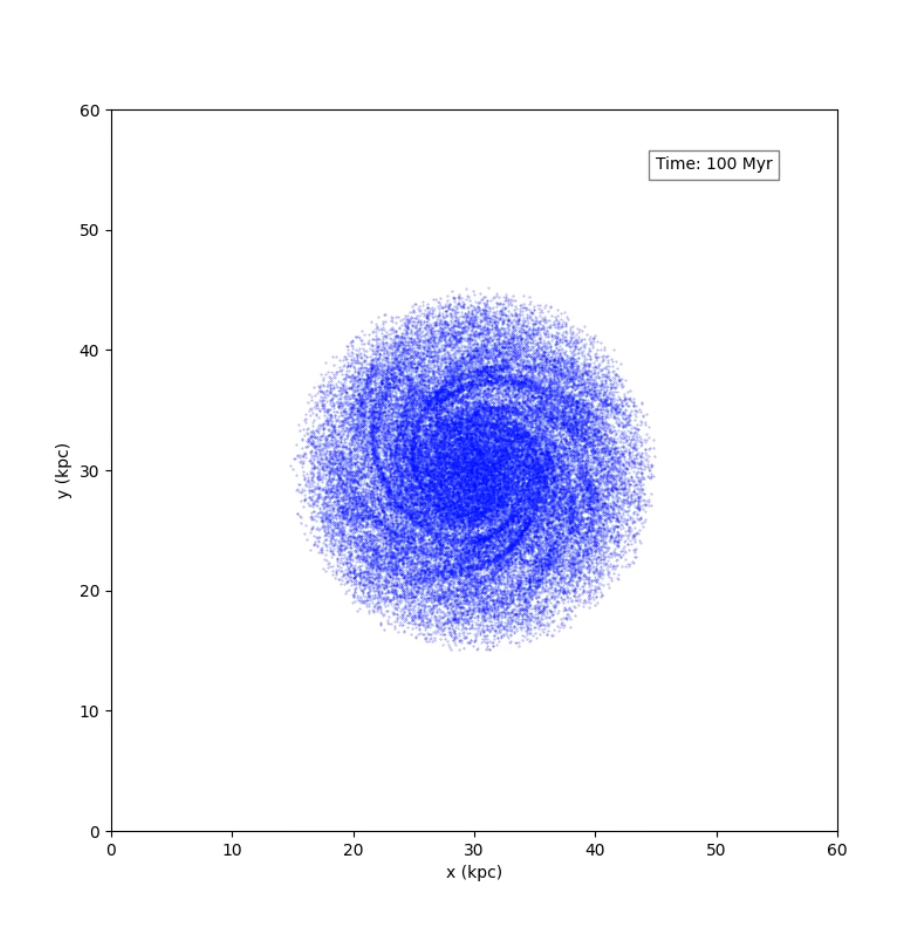
\includegraphics[width=\textwidth]{img/pm/100myr.png}
        \caption{$t=100\,\text{Myr}$}
        \label{fig:spiral-galaxy-evolution-pm-sub2}
    \end{subfigure}

    \vspace{0.5cm}

    \begin{subfigure}[b]{0.45\textwidth}
        \centering
        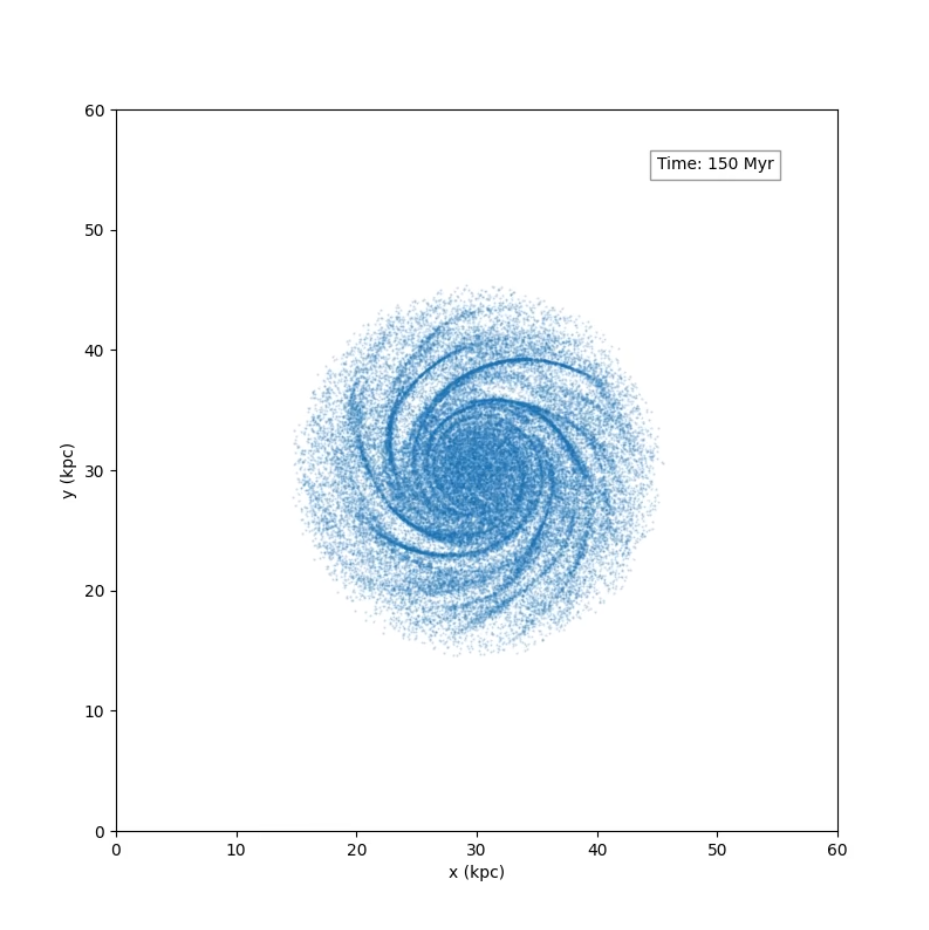
\includegraphics[width=\textwidth]{img/pm/150myr.png}
        \caption{$t=150\,\text{Myr}$}
        \label{fig:spiral-galaxy-evolution-pm-sub3}
    \end{subfigure}
    \hfill
    \begin{subfigure}[b]{0.45\textwidth}
        \centering
        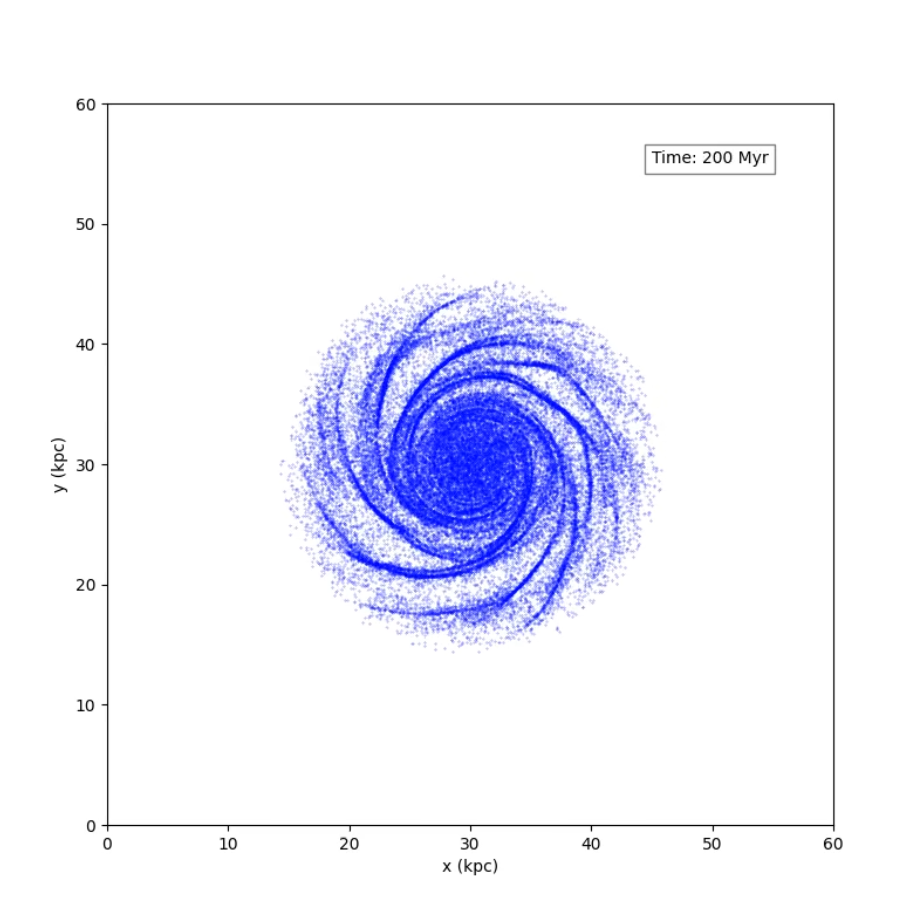
\includegraphics[width=\textwidth]{img/pm/200myr.png}
        \caption{$t=200\,\text{Myr}$}
        \label{fig:spiral-galaxy-evolution-pm-sub4}
    \end{subfigure}

    \caption{Evolution of a spiral galaxy as predicted by the PM method.}
    \label{fig:spiral-galaxy-evolution-pm}
\end{figure}

During the simulation, total energy $E = \textrm{KE} + \textrm{PE}$, angular momentum $\mathbf{l}$, and the $z$-component of the momentum vector $\mathbf{p}$ should stay constant.
The $x$- and $y$-components of momentum change due to the presence of an external gravitational field (representing the halo).
We can verify if this variation satisfies the expected relation
\begin{equation}\label{eq:expected-momentum-change}
    \dot{\mathbf{p}} = \mathbf{F}^\text{ext}
\end{equation}
by finding the initial total momentum $\mathbf{p}(t = 0)$ and incrementing the value of $\mathbf{p}$ in each time-step by $\mathbf{F}^\text{ext}\textrm{DT}$.

The exact calculation of the potential energy \cite{taylor2005classical} using the formula
\begin{equation*}
    \textrm{PE} = -\sum_{i=1}^{N}\sum_{j=i+1}^{N}\frac{G m_i m_j}{r_{ij}}
\end{equation*}
is computationally infeasible considering the $O(N^2)$ cost.
An approximation based on the potential values at mesh points,
\begin{equation*}
    \textrm{PE} \approx \frac{V}{2}\sum_{\mathbf{p}} \rho(\mathbf{x}_\mathbf{p})\phi(\mathbf{x}_\mathbf{p}),
\end{equation*}
is used instead (for derivation refer to \cite{Hockney1988}).
\begin{figure}[htp]
    \centering
    \begin{subfigure}[b]{0.45\textwidth}
        \centering
        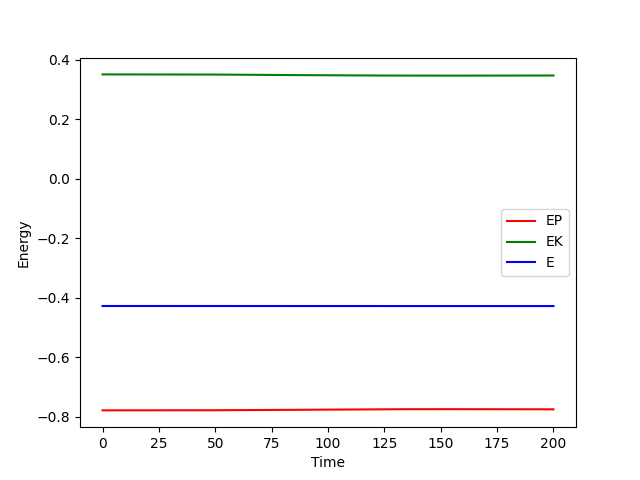
\includegraphics[width=\textwidth]{img/pm/energy.png}
        \caption{Energy}
        \label{fig:physical-quantities-pm-sub1}
    \end{subfigure}
    \hfill
    \begin{subfigure}[b]{0.45\textwidth}
        \centering
        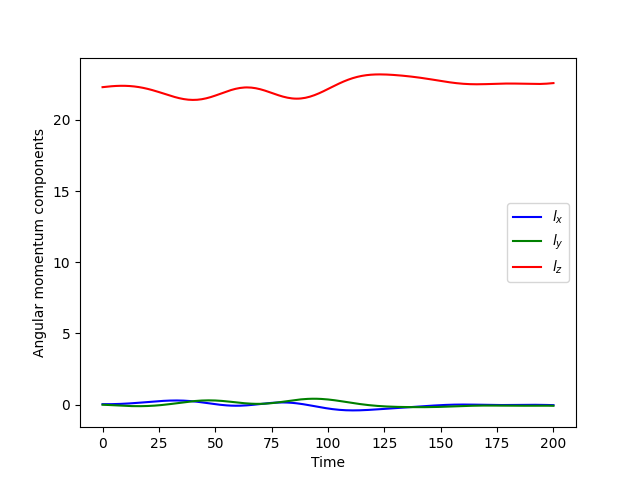
\includegraphics[width=\textwidth]{img/pm/angular-momentum.png}
        \caption{Angular momentum}
        \label{fig:physical-quantities-pm-sub2}
    \end{subfigure}

    \vspace{0.5cm}

    \begin{subfigure}[b]{0.45\textwidth}
        \centering
        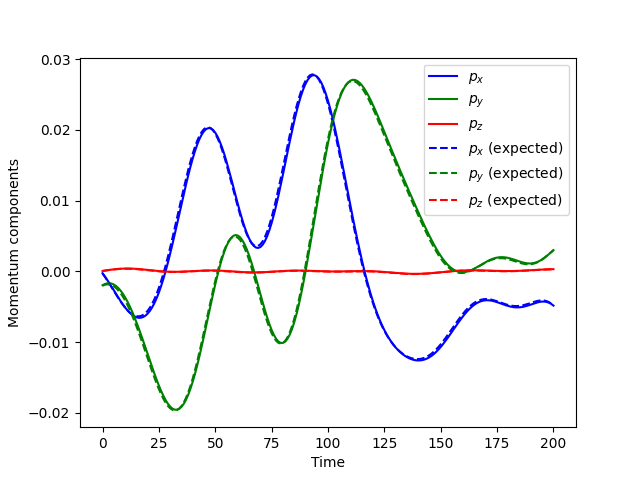
\includegraphics[width=\textwidth]{img/pm/momentum.png}
        \caption{Momentum; broken lines represent the expected momentum following \autoref{eq:expected-momentum-change}}
        \label{fig:physical-quantities-pm-sub3}
    \end{subfigure}

    \caption{Fundamental physical quantities describing the system over time in the PM simulation.
        Time is in Myr and the quantities are expressed in units consistent with \autoref{tab:galaxy-parameters}}
    \label{fig:physical-quantities-pm}
\end{figure}

\subsection{Particle-particle particle-mesh method}
The \PThreeM{} based simulation uses the same parameters as the PM method.
The reference force was calculated using the $S_1$ shape formula (\autoref{eq:s1-reference-force}) with particle diameter $a=3H$.
The cutoff radius was set to $r_e=0.7a$.
One extra free parameter is the \textit{softening length} $\epsilon$ which modifies the universal law of gravitation so that division by zero can be avoided, i.e. the modified law is
\begin{equation*}
    F^\text{soft}_{ij}(r) = \frac{G m_i m_j}{r_{ij}^2 + \epsilon^2}.
\end{equation*}
In the simulation, $\epsilon$ was set arbitrarily to $1.5$ kpc.
The system's evolution is presented in \autoref{fig:spiral-galaxy-evolution-p3m}.
\begin{figure}[htp]
    \centering
    \begin{subfigure}[b]{0.45\textwidth}
        \centering
        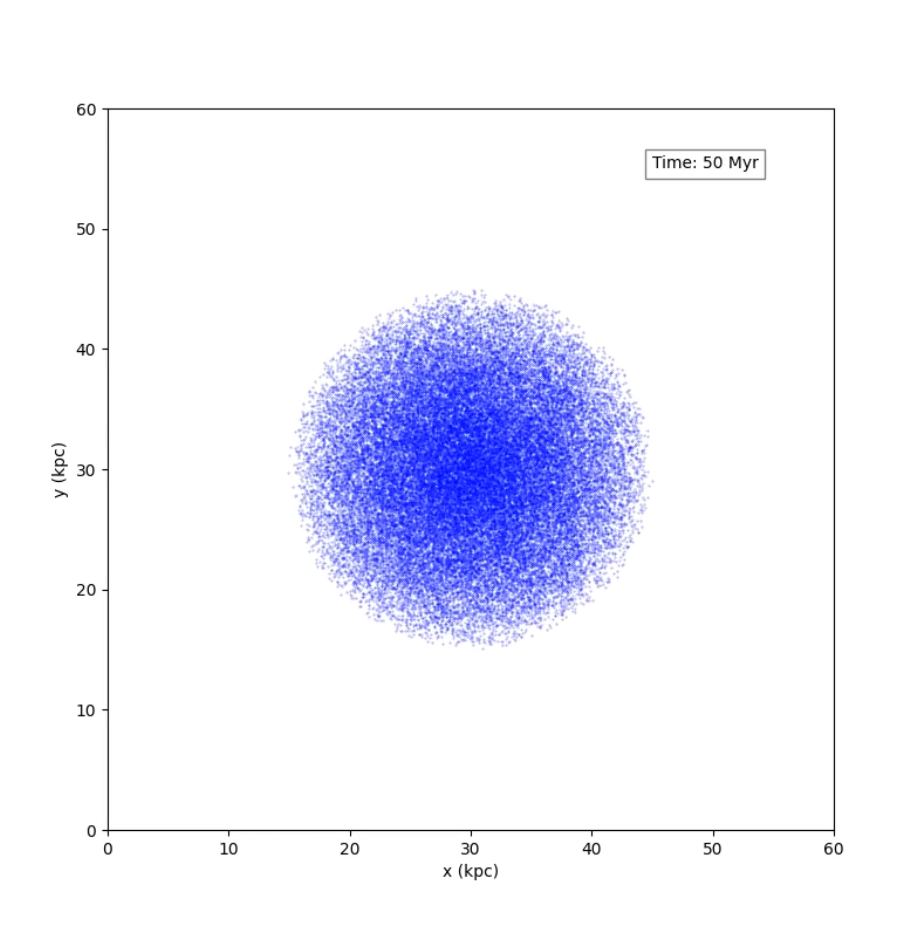
\includegraphics[width=\textwidth]{img/p3m/50myr.png}
        \caption{$t=50\,\text{Myr}$}
        \label{fig:spiral-galaxy-evolution-p3m-sub1}
    \end{subfigure}
    \hfill
    \begin{subfigure}[b]{0.45\textwidth}
        \centering
        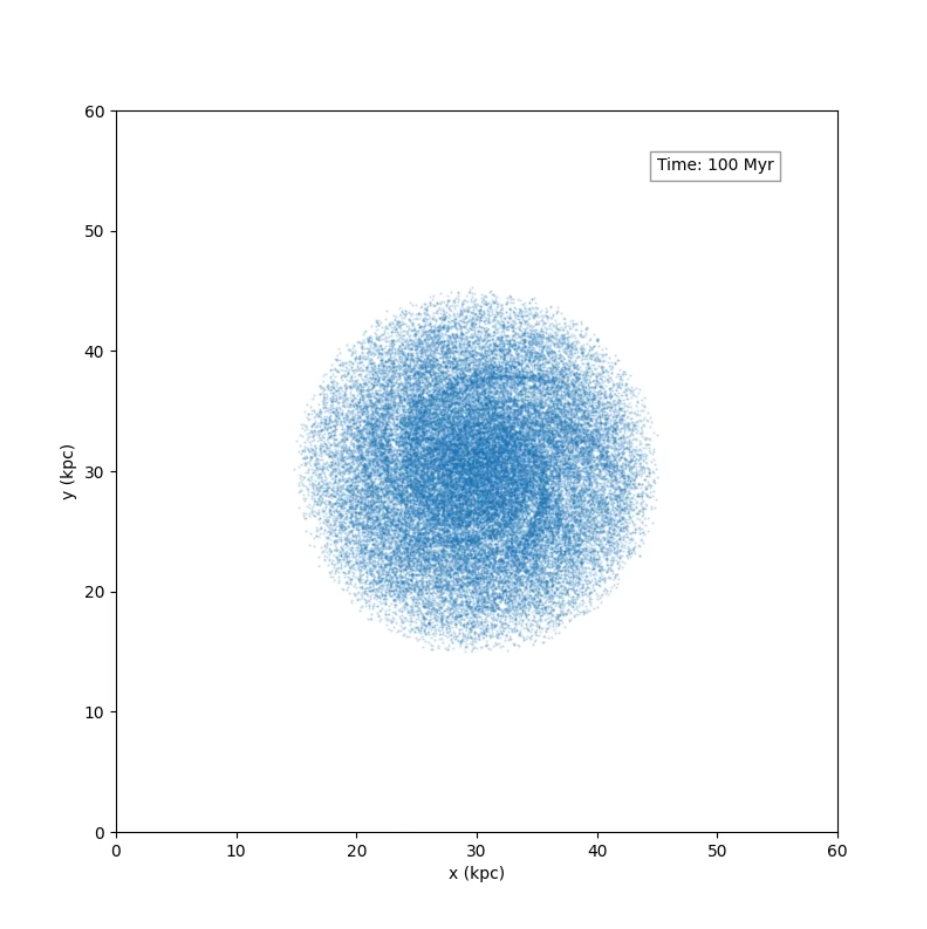
\includegraphics[width=\textwidth]{img/p3m/100myr.png}
        \caption{$t=100\,\text{Myr}$}
        \label{fig:spiral-galaxy-evolution-p3m-sub2}
    \end{subfigure}

    \vspace{0.5cm}

    \begin{subfigure}[b]{0.45\textwidth}
        \centering
        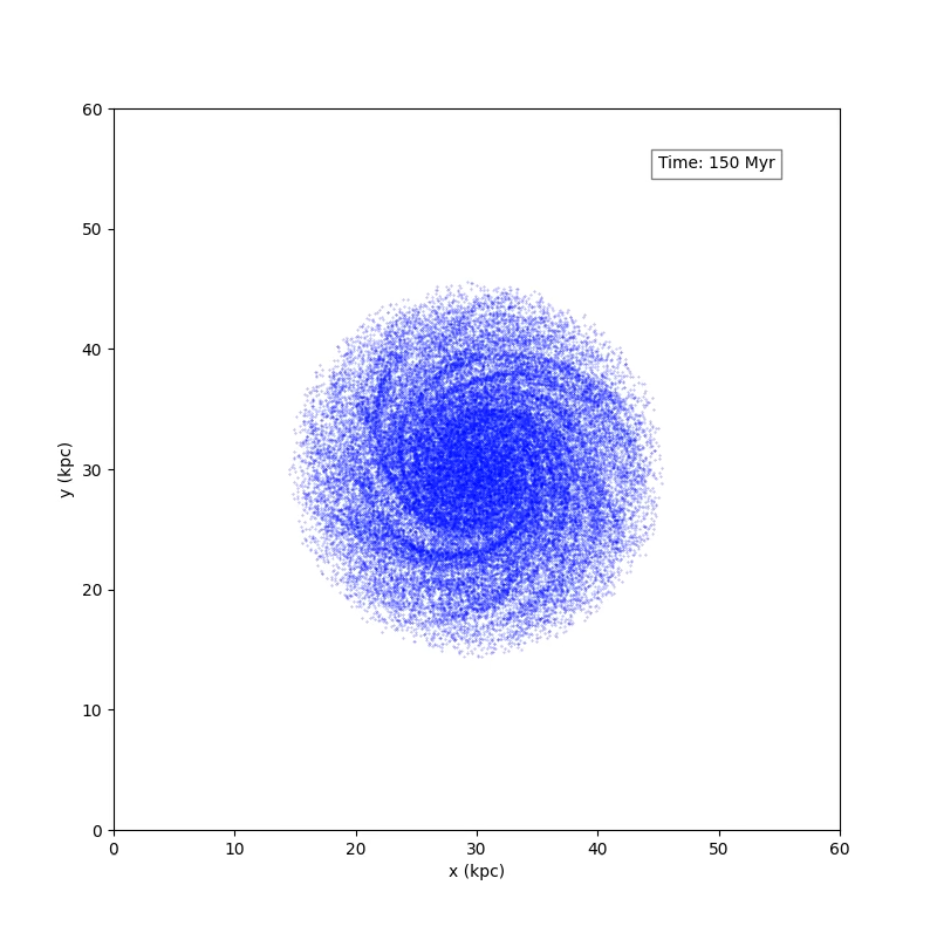
\includegraphics[width=\textwidth]{img/p3m/150myr.png}
        \caption{$t=150\,\text{Myr}$}
        \label{fig:spiral-galaxy-evolution-p3m-sub3}
    \end{subfigure}
    \hfill
    \begin{subfigure}[b]{0.45\textwidth}
        \centering
        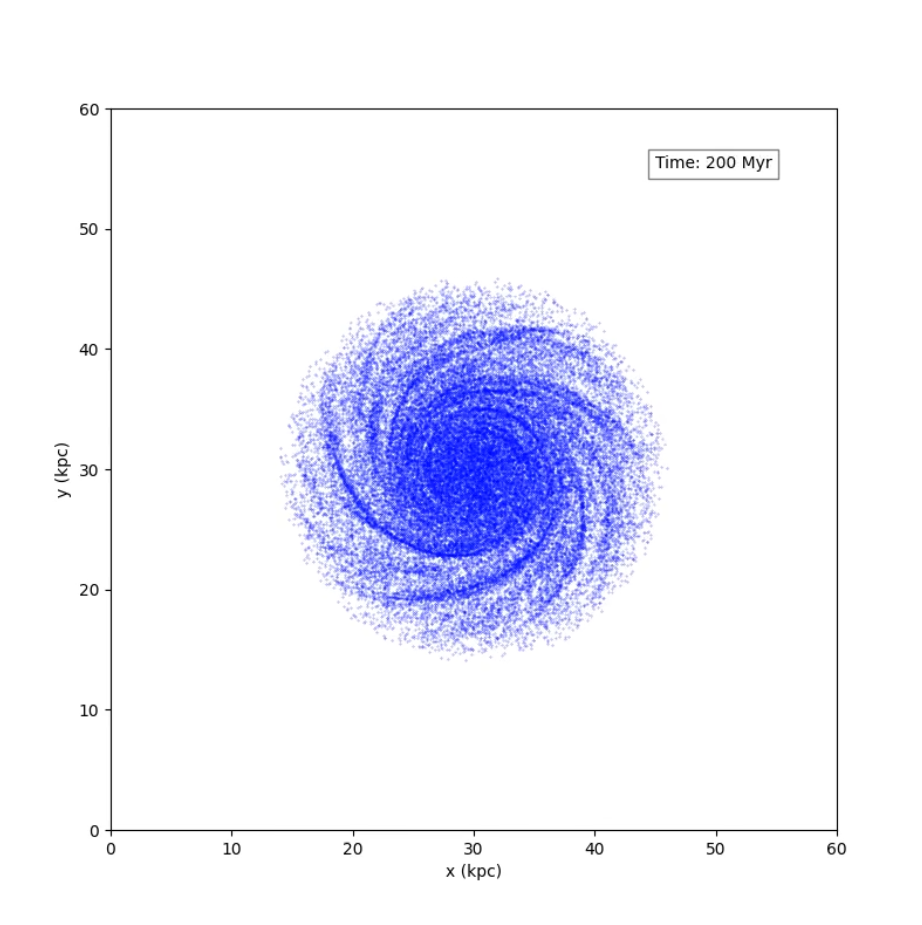
\includegraphics[width=\textwidth]{img/p3m/200myr.png}
        \caption{$t=200\,\text{Myr}$}
        \label{fig:spiral-galaxy-evolution-p3m-sub4}
    \end{subfigure}

    \caption{Evolution of a spiral galaxy as predicted by the \PThreeM{} method.}
    \label{fig:spiral-galaxy-evolution-p3m}
\end{figure}
Graphs of energy, angular momentum, and momentum components vs. time are shown in \autoref{fig:physical-quantities-p3m}.
\begin{figure}[htp]
    \centering
    \begin{subfigure}[b]{0.45\textwidth}
        \centering
        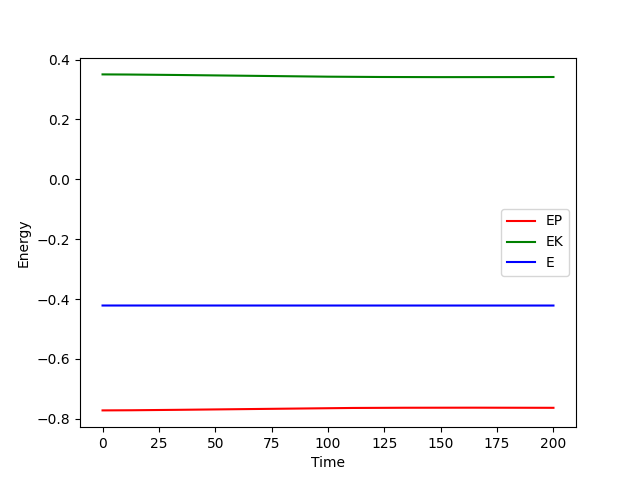
\includegraphics[width=\textwidth]{img/p3m/energy.png}
        \caption{Energy}
        \label{fig:physical-quantities-p3m-sub1}
    \end{subfigure}
    \hfill
    \begin{subfigure}[b]{0.45\textwidth}
        \centering
        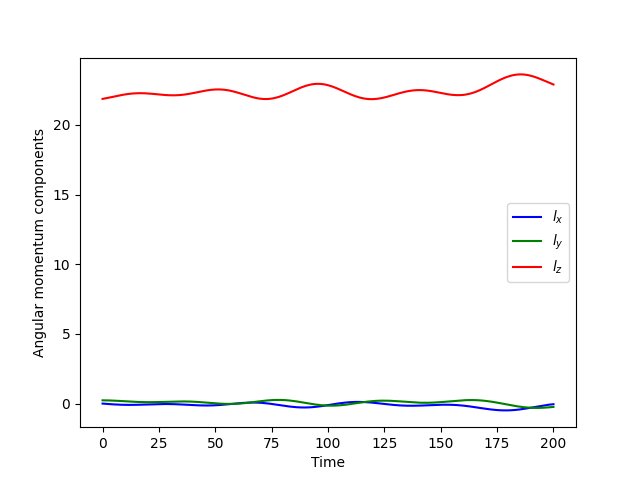
\includegraphics[width=\textwidth]{img/p3m/angular-momentum.png}
        \caption{Angular momentum}
        \label{fig:physical-quantities-p3m-sub2}
    \end{subfigure}

    \vspace{0.5cm}

    \begin{subfigure}[b]{0.45\textwidth}
        \centering
        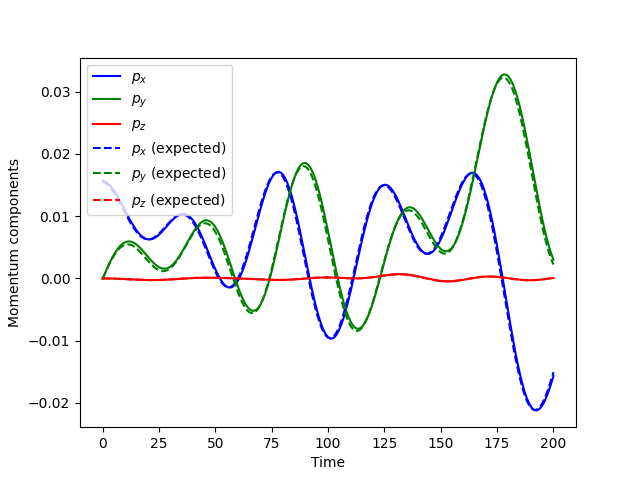
\includegraphics[width=\textwidth]{img/p3m/momentum.png}
        \caption{Momentum; broken lines represent the expected momentum following \autoref{eq:expected-momentum-change}}
        \label{fig:physical-quantities-p3m-sub3}
    \end{subfigure}

    \caption{Fundamental physical quantities describing the system over time in the \PThreeM{} simulation.
        Time is in Myr and the quantities are expressed in units consistent with \autoref{tab:galaxy-parameters}}
    \label{fig:physical-quantities-p3m}
\end{figure}

\subsection{Performance analysis}
The PM and \PThreeM{} methods were implemented exactly as described in the previous sections.
The PM method was developed for both CPU and GPU architectures, using C++ and CUDA C++, respectively, while the \PThreeM{} method is currently available only in the CPU variant.
The implementation relies on external libraries for fast Fourier transform computations: FFTW for the CPU version and cuFFT for the GPU version.
A performance comparison of the PM method was conducted using $N = 2^{16} = 65,536$ particles on a $64 \times 64 \times 64$ mesh with the CIC assignment scheme.
The tests were run on a system equipped with an Intel(R) Core(TM) i7-9750H CPU @ 2.60GHz and an NVIDIA GeForce GTX 1650 GPU. Over 200 iterations, the CPU implementation consistently took around 2.3 seconds, while the GPU implementation reduced this to approximately 1.0 second (excluding data transfer time between host and device).
Notably, the most time-consuming part of the program was unrelated to computation—writing data to disk in text format took nearly 20 seconds.

For the \PThreeM{} method, performance was measured using $N=50,000$ particles on a $128 \times 128 \times 64$ mesh with the TSC assignment scheme.
The total runtime was approximately 1 minute and 30 seconds, with the time distribution among key algorithm components as follows:
\begin{itemize}
    \item HOC table initialization: 12\%
    \item Short-range force calculations: 80\%
    \item PM step: 7.5\%
\end{itemize}
The code is available at \url{https://github.com/AleksyBalazinski/ParticleSimulation} under the MIT license.

\bibliographystyle{plain}
\bibliography{refs}


\end{document}